% \documentclass[letterpaper]{article}
%DIF LATEXDIFF DIFFERENCE FILE
%DIF DEL Original/main.tex   Fri Jun 16 17:23:12 2023
%DIF ADD Revision/main.tex   Mon Jun 19 20:43:43 2023
% \usepackage[english]{babel}
% \usepackage[utf8]{inputenc}
% \usepackage[top=1.2in, left=0.9in, bottom=1.2in, right=0.9in]{geometry} % sets the margins
% \usepackage{amsmath,amsthm,amssymb}
% \usepackage{url} % fixes url problem
% \usepackage{csquotes}% Recommended
% \usepackage[doublespacing]{setspace} % turns on double spacing
% \usepackage{multirow}
% \usepackage{caption}
% \usepackage{subcaption}
% \captionsetup{compatibility=false}
% \usepackage{graphicx}
% \usepackage[table]{xcolor}

% \bibliographystyle{abbrv}

% Adding commands for Atmospheric Chemistry and Physics here
\documentclass[journal abbreviation, manuscript]{copernicus}
\newcounter{algorithm} %DIF > 
%DIF PREAMBLE EXTENSION ADDED BY LATEXDIFF
%DIF UNDERLINE PREAMBLE %DIF PREAMBLE
\RequirePackage[normalem]{ulem} %DIF PREAMBLE
\RequirePackage{color}\definecolor{RED}{rgb}{1,0,0}\definecolor{BLUE}{rgb}{0,0,1} %DIF PREAMBLE
\providecommand{\DIFadd}[1]{{\protect\color{blue}\uwave{#1}}} %DIF PREAMBLE
\providecommand{\DIFdel}[1]{{\protect\color{red}\sout{#1}}}                      %DIF PREAMBLE
%DIF SAFE PREAMBLE %DIF PREAMBLE
\providecommand{\DIFaddbegin}{} %DIF PREAMBLE
\providecommand{\DIFaddend}{} %DIF PREAMBLE
\providecommand{\DIFdelbegin}{} %DIF PREAMBLE
\providecommand{\DIFdelend}{} %DIF PREAMBLE
\providecommand{\DIFmodbegin}{} %DIF PREAMBLE
\providecommand{\DIFmodend}{} %DIF PREAMBLE
%DIF FLOATSAFE PREAMBLE %DIF PREAMBLE
\providecommand{\DIFaddFL}[1]{\DIFadd{#1}} %DIF PREAMBLE
\providecommand{\DIFdelFL}[1]{\DIFdel{#1}} %DIF PREAMBLE
\providecommand{\DIFaddbeginFL}{} %DIF PREAMBLE
\providecommand{\DIFaddendFL}{} %DIF PREAMBLE
\providecommand{\DIFdelbeginFL}{} %DIF PREAMBLE
\providecommand{\DIFdelendFL}{} %DIF PREAMBLE
%DIF LISTINGS PREAMBLE %DIF PREAMBLE
\RequirePackage{listings} %DIF PREAMBLE
\RequirePackage{color} %DIF PREAMBLE
\lstdefinelanguage{DIFcode}{ %DIF PREAMBLE
%DIF DIFCODE_UNDERLINE %DIF PREAMBLE
  moredelim=[il][\color{red}\sout]{\%DIF\ <\ }, %DIF PREAMBLE
  moredelim=[il][\color{blue}\uwave]{\%DIF\ >\ } %DIF PREAMBLE
} %DIF PREAMBLE
\lstdefinestyle{DIFverbatimstyle}{ %DIF PREAMBLE
	language=DIFcode, %DIF PREAMBLE
	basicstyle=\ttfamily, %DIF PREAMBLE
	columns=fullflexible, %DIF PREAMBLE
	keepspaces=true %DIF PREAMBLE
} %DIF PREAMBLE
\lstnewenvironment{DIFverbatim}{\lstset{style=DIFverbatimstyle}}{} %DIF PREAMBLE
\lstnewenvironment{DIFverbatim*}{\lstset{style=DIFverbatimstyle,showspaces=true}}{} %DIF PREAMBLE
%DIF END PREAMBLE EXTENSION ADDED BY LATEXDIFF

\begin{document}

\title{Molecular simulations reveal that heterogeneous ice nucleation occurs at higher temperatures in water under capillary tension}
% Molecular simulations quantify the increase of heterogeneous ice nucleation temperature in water under capillary tension


% \author{Elise Rosky, Will Cantrell, Tianshu Li, Issei Nakamura, Raymond A. Shaw}
% \date{\today}

\Author[1]{Elise}{Rosky}
\Author[1]{Will}{Cantrell}
\Author[2]{Tianshu}{Li}
\Author[1]{Issei}{Nakamura}
\Author[1]{Raymond A.}{Shaw}

\affil[1]{Department of Physics, Michigan Technological University, Houghton, MI, USA}
\affil[2]{Department of Civil \& Environmental Engineering, George Washington University, Washington, DC, USA}

\correspondence{Elise Rosky (emrosky@mtu.edu)}

\runningtitle{Heterogeneous ice nucleation in water under capillary tension}

\runningauthor{Rosky et al.}


\received{}
\pubdiscuss{} %% only important for two-stage journals
\revised{}
\accepted{}
\published{}

%% These dates will be inserted by Copernicus Publications during the typesetting process.


\firstpage{1}

\maketitle

%\begin{document}
%\maketitle

%\section{Abstract}

\begin{abstract}
%  After a brief introduction of the topic, the summary recapitulates the key points of the article and mentions possible directions for prospective research. 

Homogeneous ice nucleation rates occur at higher temperatures when water is under tension, otherwise referred to as negative pressure. If also true for heterogeneous ice nucleation rates, then this phenomenon can result in higher heterogeneous freezing temperatures in water capillary bridges, pores, and other geometries where water is subjected to negative Laplace pressure. Using a molecular model of water \DIFdelbegin \DIFdel{freezing on a hydrophilic substrate, it is found that }\DIFdelend \DIFaddbegin \DIFadd{that is freezing on an ice-nucleating substrate; }\DIFaddend heterogeneous ice nucleation rates exhibit a similar temperature increase at negative pressures as homogeneous ice nucleation. For pressures ranging from \DIFdelbegin \DIFdel{from 1 }\DIFdelend \DIFaddbegin \DIFadd{$1$ }\DIFaddend atm to $-1000$ atm, the simulations reveal that the temperature corresponding to the heterogeneous nucleation rate coefficient $j_{het}$ (m$^{-2}$ s$^{-1}$) increases \DIFdelbegin \DIFdel{linearly }\DIFdelend as a function of negative pressure\DIFdelbegin \DIFdel{, with a slope that can be approximately predicted by the water density anomaly }\DIFdelend \DIFaddbegin \DIFadd{. In the negative pressure regime, the slope of the temperature increase with decreasing pressure can be approximated as linear, with steepness of the slope influenced by the density difference between liquid and ice, }\DIFaddend and the latent heat of fusion at atmospheric pressure.

Simulations of water in capillary bridges confirm that negative Laplace pressure within the water corresponds to an increase in heterogeneous freezing temperature. The freezing temperature in the water capillary bridges increases linearly with inverse capillary height ($1/h$). Varying the height and width of the capillary bridge \DIFdelbegin \DIFdel{reveals the role of geometric factors in }\DIFdelend \DIFaddbegin \DIFadd{elucidates the influence geometric factors can have on }\DIFaddend heterogeneous ice nucleation. When \DIFdelbegin \DIFdel{substrate surfaces are separated by }\DIFdelend \DIFaddbegin \DIFadd{the height of the capillary bridge is }\DIFaddend less than approximately $h$ = 20 \AA{} the nucleation rate is enhanced \DIFdelbegin \DIFdel{and when }\DIFdelend \DIFaddbegin \DIFadd{due to confinement between the substrate surfaces. When }\DIFaddend the width of the capillary bridge is less than approximately 30 \AA{} the nucleation rate is suppressed\DIFdelbegin \DIFdel{. Ice nucleation does not occur in the region within }\DIFdelend \DIFaddbegin \DIFadd{, perhaps resulting from the apparent lack of ice nucleation within $\sim$}\DIFaddend 10 \AA{} of the air-water interface\DIFdelbegin \DIFdel{and shows a preference for nucleation in the region just beyond 10 \AA{}}\DIFdelend .

These results help unify multiple lines of experimental evidence for enhanced nucleation rates due to reduced pressure, either resulting from surface geometry (Laplace pressure) or mechanical agitation of water droplets. This concept is relevant to the phenomenon of contact nucleation and could potentially play a role in a number of different heterogeneous nucleation or secondary ice mechanisms. \DIFaddbegin \DIFadd{The linear approximation presented is appropriate for use in the negative pressure regime, providing a simple estimate of the heterogeneous freezing temperature increase in water due to negative Laplace pressure.
}\DIFaddend 

%"In the context of atmospheric ice-nucleating particles, our results strongly support the experimental evidence for the importance of surface features and dynamic processes that can initiate ice nucleation at low supercooling."
% disclaimer the structure of the above sentence is extremely similar and arguably plaigerized from the abstract of Roudsari et al. 2022 (https://doi.org/10.5194/acp-22-10099-2022)
% I just really like how they stated it and think we could add a similar statement of relevance to atmospheric INP.
\end{abstract}


%\section{Introduction}
\introduction

Heterogeneous freezing of water occurs when a substrate or material in contact with water catalyzes the formation of ice. The heterogeneous ice nucleation rate coefficient, referred to in this paper as the intensive nucleation rate $j_{het}$, describes the number of ice nucleation events per unit area of substrate per unit time (m$^{-2}$ s$^{-1}$). It is commonly recognized that $j_{het}$ is temperature dependent, with \DIFdelbegin \DIFdel{increasing }\DIFdelend probability of nucleation \DIFaddbegin \DIFadd{increasing }\DIFaddend as temperature is decreased. Meanwhile, less attention has been given to the pressure dependence of $j_{het}$, which will be the focus of this study. \DIFaddbegin \DIFadd{Specifically, we study the behavior of $j_{het}$ under negative pressure, with the hypothesis being that negative pressure in supercooled water will correspond to elevated temperatures of heterogeneous ice nucleation.
}

\DIFaddend Negative pressure in water is prevalent throughout nature, occurring in tree xylem \citep{jacobsen2007xylem}, in water capillary bridges in soil \citep{seiphoori2020}, and within nano-sized pores on atmospheric ice nucleating particles \citep{david2020role,marcolli2020technical,klumpp2023comparing}. Negative Laplace pressure, given by $\Delta P \approx \sigma_{lv}/2r$, \DIFaddbegin \DIFadd{(}\DIFaddend where $\sigma_{lv} \approx 0.7$ J m$^{-2}$  is the liquid-vapor surface tension of water\DIFaddbegin \DIFadd{)}\DIFaddend , becomes significant for nucleation when the air-water interface radius of curvature $r$ is on the order of nanometers\DIFdelbegin \DIFdel{, leading }\DIFdelend \DIFaddbegin \DIFadd{. This corresponds }\DIFaddend to negative pressures \DIFdelbegin \DIFdel{of order 100s }\DIFdelend \DIFaddbegin \DIFadd{on the  order of  hundreds }\DIFaddend of atmospheres. Thus, in this work we explore atmospherically-relevant negative pressures down to $-1000$ atm. %These nanometer length scales are essential to processes such as the condensation of water into pores in cirrus clouds \cite{robert2019} and may also be relevant to ice nucleation on atmospheric substrates as well.

\DIFaddbegin \DIFadd{Though small changes in temperature exert a much larger influence on ice nucleation rate compared to changes in pressure, our results show that negative pressures within the range of $-1000$ atm can cause heterogeneous ice nucleation rates to occur several Kelvin higher compared to without any pressure change. Within the narrow band of temperatures where heterogeneous ice nucleation is active in the atmosphere, it is commonly approximated that the concentration of ice-nucleating particles increases exponentially with decreasing temperature \mbox{%DIFAUXCMD
\citep[Sec. 9.2]{pruppacher1997}}\hspace{0pt}%DIFAUXCMD
; this suggests the activation of ice-nucleating particles a few Kelvin warmer can have significant impacts.
}

\DIFaddend Recent experiments provide compelling evidence that dynamic or geometric factors can lead to \DIFdelbegin \DIFdel{enhancements of the nucleation rate }\DIFdelend \DIFaddbegin \DIFadd{enhancement of ice nucleation rates }\DIFaddend independent of temperature\DIFaddbegin \DIFadd{, leading investigators to explore non-thermal sources of freezing enhancement}\DIFaddend . For example, it is widely known that contact between an ice-nucleating material and supercooled liquid leads to an increase in the freezing temperature \DIFaddbegin \DIFadd{as }\DIFaddend compared to when the material is immersed \citep{pitter1973wind,levin1983contact,diehl2002ice}. Wetting of a small ice-nucleating particle at a water surface \citep{shaw2005} and roughening of a substrate \citep{gurganus2014nucleation} \DIFdelbegin \DIFdel{both have been observed to yield }\DIFdelend \DIFaddbegin \DIFadd{have both yielded }\DIFaddend similar increases. Even contact with a soluble material not typically considered an ice nucleating particle can induce freezing \citep{niehaus2015}. It has been observed that ice nucleation is strongly enhanced when the three-phase contact line of a sessile drop distorts and moves over a substrate during electrowetting \citep{yang2015} or over a surface with pinning points \citep{yang2018}. One hypothesis that attempts to unify these diverse observations is that the curvature and/or stretching of the air-water interface produces negative Laplace pressure and tension within the water \citep{marcolli2017,yang2020}.

%There is evidence that negative pressure, also referred to as tension, increases ice nucleation rates in supercooled water. As hypothesized by Yang et al. (2018, 2020) and Marcolli (2017), this phenomenon could potentially explain laboratory results that show higher freezing temperatures in water droplets that are subjected to stretching and distorting of the droplet surface (the air-water interface) \cite{marcolli2017, yang2015,yang2018,niehaus2015,yang2020,shaw2005}. The curvature and stretching at the air-water interface is thought to produce negative Laplace pressure and tension within the water. 

Our previous molecular dynamics simulations of \DIFaddbegin \DIFadd{homogeneous }\DIFaddend ice nucleation within pure water \DIFdelbegin \DIFdel{(homogeneous ice nucleation) }\DIFdelend identified that homogeneous ice nucleation rates occur at higher temperatures due to negative pressure, \DIFdelbegin \DIFdel{with }\DIFdelend \DIFaddbegin \DIFadd{where }\DIFaddend the increase in temperature $\Delta T$ resulting from a decrease in pressure $\Delta P$ \DIFaddbegin \DIFadd{is }\DIFaddend described by the linear approximation \citep{rosky2022}

\begin{equation} \label{eq:dTdP}
    \Delta T = \frac{T_m \Delta \nu_{ls}}{l_f} \Delta P.
\end{equation}

\noindent The governing quantities are the equilibrium melting point ($T_m$), the molar-volume difference between liquid and solid water ($\Delta \nu_{ls}$), and the enthalpy of fusion (also known as latent heat, $l_f$) --- all evaluated at a reference pressure of 1 atmosphere. The molar volume difference between water and ice is negative \DIFdelbegin \DIFdel{, a property more commonly known as the water density anomaly. An }\DIFdelend \DIFaddbegin \DIFadd{across the range of pressures addressed in this study. This property of water allows for an }\DIFaddend increase in freezing temperature ($\Delta T > 0$) from a decrease in pressure ($\Delta P < 0$)\DIFdelbegin \DIFdel{is made possible by this property of water}\DIFdelend . A thorough derivation of Eq. (\ref{eq:dTdP}) can be found in the appendix of \citet{rosky2022}, using the pressure-dependent formulation of the solid-liquid chemical potential difference ($\mu$) formulated by \citet{nemec2013} combined with classical nucleation theory for $j_{hom}$ \citep[see also][]{yang2018}. \DIFdelbegin \DIFdel{According to this approximation}\DIFdelend \DIFaddbegin \DIFadd{Several thermodynamic properties of water such as the liquid density, latent heat of fusion, and ice--liquid surface tension are all approximated as constant with temperature and pressure on the scales relevant to this work.
}

\DIFadd{According to the approximation of Equation \ref{eq:dTdP}}\DIFaddend , the slope of \DIFdelbegin \DIFdel{$\Delta T/\Delta P$ }\DIFdelend \DIFaddbegin \DIFadd{$(\Delta T/\Delta P)_{hom}$ }\DIFaddend is parallel to the liquid-solid phase coexistence \DIFaddbegin \DIFadd{(melting point) }\DIFaddend line, given by the Clapeyron equation. \DIFdelbegin \DIFdel{Detailed studies support }\DIFdelend \DIFaddbegin \DIFadd{It is important to note }\DIFaddend that the slope of \DIFaddbegin \DIFadd{the }\DIFaddend homogeneous freezing lines \DIFdelbegin \DIFdel{is }\DIFdelend \DIFaddbegin \DIFadd{are }\DIFaddend not actually parallel to the melting point line \DIFdelbegin \DIFdel{\mbox{%DIFAUXCMD
\citep{bianco2021, espinosa2016}}\hspace{0pt}%DIFAUXCMD
, but }\DIFdelend \DIFaddbegin \DIFadd{as shown in both experiments and simulations of water  \mbox{%DIFAUXCMD
\citep{bianco2021, espinosa2016, kanno1975, lu2016anomaly, dhabal2022icewater}}\hspace{0pt}%DIFAUXCMD
. In particular, the slope of $(\Delta T/\Delta P)_{hom}$ becomes increasingly steeper than the melting point line at large positive pressures. However, all of these studies suggest that the homogeneous freezing line and melting point line become closer in slope when approaching the negative pressure regime. Indeed, }\DIFaddend \citet{rosky2022} has shown that \DIFdelbegin \DIFdel{, as an approximation, it holds true for }\DIFdelend \DIFaddbegin \DIFadd{approximating the two slopes as parallel is satisfactory at negative }\DIFaddend pressures ranging from 1 atm to \DIFdelbegin \DIFdel{-1000 atm. }\DIFdelend \DIFaddbegin \DIFadd{$-1000$ atm. Furthermore, inspection of the simulated thermodynamic properties of water by \mbox{%DIFAUXCMD
\citet{MonteroDeHijes2023} }\hspace{0pt}%DIFAUXCMD
arrived at a similar conclusion that ``the homogeneous nucleation line should be parallel to the coexistence line for pressures below 500 $\sim$bars.'' }\DIFaddend In the present study we ask: Does the heterogeneous ice nucleation rate follow a similar expression for pressure dependence \DIFdelbegin \DIFdel{as }\DIFdelend \DIFaddbegin \DIFadd{in the negative pressure regime as does }\DIFaddend the homogeneous ice nucleation rate? And do simple geometric arrangements leading to negative Laplace pressure indeed result in similar behavior?

The behavior of homogeneous ice nucleation at negative pressures has been the subject of investigation because of its relationship to the fundamental properties of water \DIFdelbegin \DIFdel{\mbox{%DIFAUXCMD
\citep[e.g.,][]{bianco2021}}\hspace{0pt}%DIFAUXCMD
. By restricting the study to only the range of negative pressures thought to be relevant to the atmosphere, the previously-mentioned molecular simulations of \mbox{%DIFAUXCMD
\citet{rosky2022} }\hspace{0pt}%DIFAUXCMD
were able }\DIFdelend \DIFaddbegin \DIFadd{\mbox{%DIFAUXCMD
\citep[e.g.,][]{bianco2021, lu2016anomaly}}\hspace{0pt}%DIFAUXCMD
. The work of \mbox{%DIFAUXCMD
\citet{rosky2022} }\hspace{0pt}%DIFAUXCMD
used molecular simulations }\DIFaddend to characterize a \DIFdelbegin \DIFdel{simpler }\DIFdelend \DIFaddbegin \DIFadd{simple }\DIFaddend (linear) behavior of homogeneous ice nucleation rate \DIFaddbegin \DIFadd{within the negative pressures range thought to be relevant to the atmosphere}\DIFaddend . Extending these studies to heterogeneous ice nucleation is an integral step towards applying these findings to physical situations. In particular, heterogeneous ice nucleation in atmospheric cloud droplets is of great interest because the majority of ice in the atmosphere forms via this mechanism \citep{cantrell2005production,hoose2012heterogeneous}. Heterogeneous ice nucleation rates determine the temperature at which primary ice particles form in clouds, which goes on to influence the cloud optical properties, lightning activity, and precipitation \citep{lamb2011physics}. 

In this work we characterize the pressure dependence of intensive heterogeneous ice nucleation rates $j_{het}$ \DIFaddbegin \DIFadd{at negative pressures }\DIFaddend using a molecular model of water in contact with \DIFdelbegin \DIFdel{a hydrophilic }\DIFdelend \DIFaddbegin \DIFadd{an ice-nucleating }\DIFaddend substrate. In the first method of applying negative pressure we use a barostat to explicitly set the pressure. In the second method we use capillary water bridges of varying heights to create a range of negative Laplace pressures. We consider whether Eq. (\ref{eq:dTdP}) remains a valid description for the pressure dependence of heterogeneous ice nucleation \DIFaddbegin \DIFadd{in the negative pressure range}\DIFaddend . In addition to analyzing heterogeneous ice nucleation rates, we also explore the spatial distribution of ice nucleation events within the water capillary bridges to \DIFdelbegin \DIFdel{see where nucleation events occur }\DIFdelend \DIFaddbegin \DIFadd{understand how confinement }\DIFaddend relative to the substrate and the air-water interface \DIFaddbegin \DIFadd{may influence our results}\DIFaddend . %This information reveals that all nucleation takes place between 3 to 7 \AA{} from the hydrophilic substrate. We also observe a trend of ice nucleation preferentially taking place at a certain distance from the water-vacuum interface.

While our simulations do not attempt to represent any specific substrate or configuration found in atmospheric or experimental ice nucleation, our findings provide insight into the extent that capillary tension and surface curvature (e.g. due to mechanical agitation) can influence heterogeneous ice nucleation rates through \DIFaddbegin \DIFadd{negative }\DIFaddend Laplace pressure.  Additionally, the spatial locations of ice nucleation relative to the substrate and to the air-water interface inform us that these length scales must be taken into account when considering ice nucleation rate enhancement via this mechanism.



% Talk about the equation that Janet Elliott 2021 has talked about regarding freezing point depression due to curved interface.

% Talk about Marcolli discussion of pressure-depended ice nucleation parameterizations.

% Some of the key physical factors at play with heterogeneous ice nucleation on the molecular scale. We aim to fill in more areas of uncertainty about the influence of interfaces with substrate and water surface geometry on ice nucleation rates. We study the effect that capillary water bridging has on ice nucleation rates within the water capillary bridge through negative laplace pressure.



\section{Methods}

Molecular dynamics (MD) simulations are carried out in LAMMPS \citep{plimpton1995} using the mW \citep{molinero2009} water model, and \DIFdelbegin \DIFdel{MLmW }\DIFdelend \DIFaddbegin \DIFadd{the ML-mW }\DIFaddend (Machine-Learning-mW) \DIFdelbegin \DIFdel{that }\DIFdelend \DIFaddbegin \DIFadd{which }\DIFaddend has a more realistic \DIFdelbegin \DIFdel{water density anomaly }\DIFdelend \DIFaddbegin \DIFadd{representation of the density difference between liquid water and ice  }\DIFaddend \citep{chan2019}. All simulations employ periodic boundary conditions along the three spatial dimensions. To observe ice nucleation, we equilibrate the water at a supercooled temperature \DIFdelbegin \DIFdel{(}\DIFdelend \DIFaddbegin \DIFadd{and then cool the water at a constant rate of 0.25 K ns$^{-1}$ until ice forms. The same cooling rate is used for all simulations in this study. The starting temperature for the cooling ramp at all pressures is }\DIFaddend 240 K for \DIFdelbegin \DIFdel{MLmW }\DIFdelend \DIFaddbegin \DIFadd{ML-mW }\DIFaddend and 225 K for mW, corresponding to 52 K and 48 K of supercooling respectively\DIFdelbegin \DIFdel{) and then cool the water at a constant rate of 0.25 K ns$^{-1}$ until ice forms}\DIFdelend \DIFaddbegin \DIFadd{, relative to the melting temperature at 1 atm}\DIFaddend . Ice is identified using the $q_6$ order parameter, where clusters of molecules with $q_6 > 0.54$ are considered to be ice \citep{steinhardt1983,lupi2014,rosky2022}. \DIFaddbegin \DIFadd{Using the same method as \mbox{%DIFAUXCMD
\citet{rosky2022}}\hspace{0pt}%DIFAUXCMD
, the freezing temperature of each cooling ramp is identified by the sharp increase in ice to liquid ratio. The steepest point on a sigmoidal fit to the ice/liquid ratio curve is used to select the nominal nucleation temperature. }\DIFaddend The cooling rate and substrate surface area used in this study allow us to observe intensive heterogeneous nucleation rates of order of magnitude $j_{het} = 10^{24}$ m$^{-2}$ s$^{-1}$. A timestep of 5 fs is used for all simulations.

Intensive nucleation rates are found by running the same cooling simulation a minimum of 20 times and recording the freezing temperature of each cooling run. These repeated cooling runs form a statistical distribution of freezing temperatures that can be divided into temperature bins with a corresponding intensive nucleation rate, $j_{het}(T)$, within each bin. Calculation of intensive nucleation rate values for this process is described in \citet{rosky2022} using the methods of \citet{zobrist2007}. The width of the temperature bins are displayed as uncertainty bounds on our data points. As determined from Poisson statistics, we report with 99\% certainty that the intensive nucleation rates shown are contained within the bounds of the temperature bin. We reference Table 2 of \citet{koop1997} to obtain the 99\% upper and lower confidence bounds for the number of freezing events observed in each temperature bin.

\begin{figure*}[t]
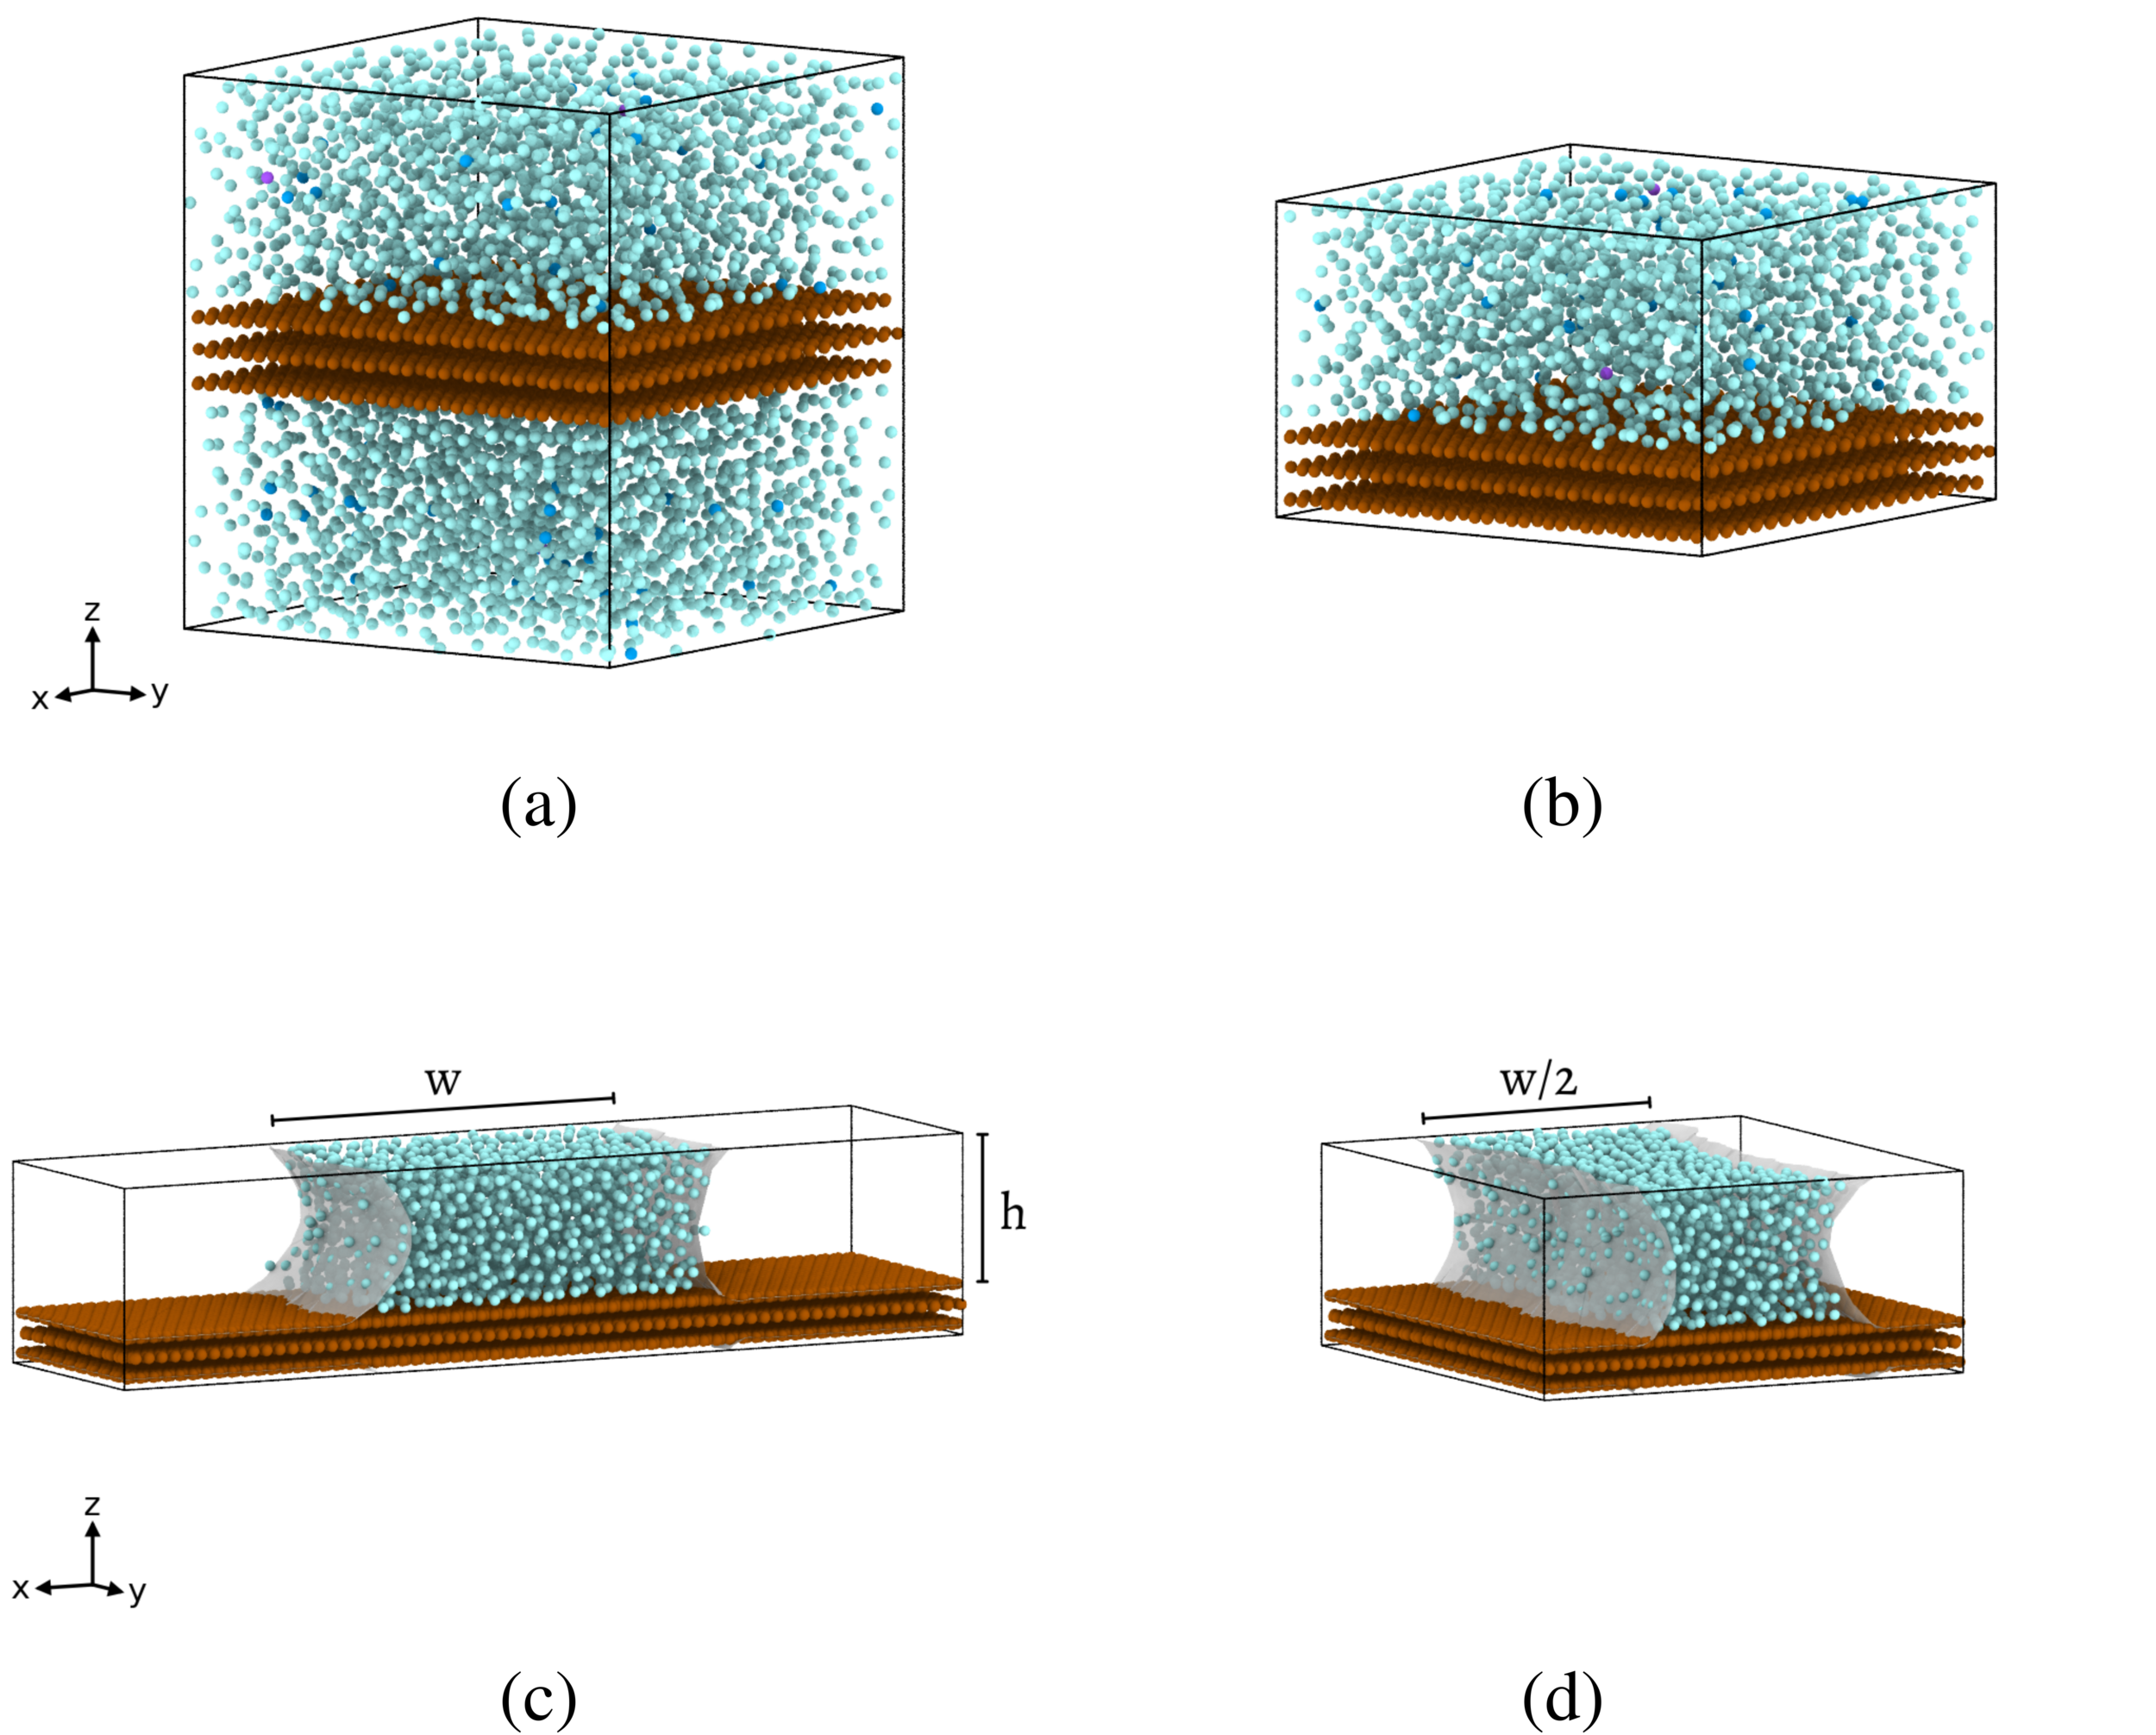
\includegraphics[width=12cm]{figures/configurations.png}
\caption{\label{fig:configurations} Heterogeneous ice nucleation simulation configurations with periodic boundary conditions employed along all three dimensions. Water molecules are cyan and the substrate material is brown. All configurations have the same total surface area of contact between water and substrate to within 6\%. (a) "Unconfined" water with a barostat. (b) Confined water with a barostat, designed to capture the effect of confining water along the $z$-axis between substrate surfaces. (c) Capillary water bridge, used without a barostat so that negative Laplace pressure may arise naturally within the water capillary bridge due to the curved geometry of the air-water interface (gray shading). (d) Narrow capillary bridge, simulates confinement of the water along the $x$-axis between the two air-water interfaces (gray shading). \DIFaddbeginFL \DIFaddFL{In configurations (b), (c), and (d), the periodic boundary conditions cause the bottom surface of the substrate to be in contact with the water molecules at the top of the simulation cell, thus forming the water bridge in (c) and (d).}\DIFaddendFL }
\end{figure*}

We simulate heterogeneous ice nucleation by inserting \DIFdelbegin \DIFdel{a hydrophilic }\DIFdelend \DIFaddbegin \DIFadd{an ice-nucleating }\DIFaddend substrate into a box of water with periodic boundary conditions. This configuration is shown in Fig. \ref{fig:configurations}(a). The substrate molecules are held fixed with zero velocity. \DIFdelbegin \DIFdel{Applying }\DIFdelend \DIFaddbegin \DIFadd{After equilibration with a Berendsen barostat (damping constant of 10000) and Bussi thermostat (damping constant of 5000), we then apply }\DIFaddend a Nose-Hoover barostat \DIFaddbegin \DIFadd{(damping constant of 10000) and Bussi thermostat }\DIFaddend to the simulation box, \DIFdelbegin \DIFdel{we }\DIFdelend \DIFaddbegin \DIFadd{and use cooling ramps to }\DIFaddend measure $j_{het}(T)$ at three pressures: 1 atm, $-500$ atm, and $-1000$ atm. The \DIFaddbegin \DIFadd{Fig. \ref{fig:configurations}(a) }\DIFaddend simulation box has dimensions of 49.22$\times$49.02$\times$58.75 \AA{}, containing 4,906 water molecules with a 10 \AA{} thick sheet of \DIFdelbegin \DIFdel{hydrophilic }\DIFdelend \DIFaddbegin \DIFadd{ice-nucleating }\DIFaddend substrate inserted at the center of the z-axis. The total surface area of the substrate in contact with water (including both the top and bottom of the substrate) is 48.25 nm$^2$. Simulations containing 4,906 molecules (a volume of roughly 125 nm$^3$) are a conventional choice for studies that aim to simulate bulk water properties \citep[e.g.,][]{molinero2009, lupi2014, li2011}. The interaction forces felt between two water molecules in our simulation go to zero when molecules are spaced further than $\sim$4 \AA{} apart, and forces between water molecules and substrate molecules go to zero for separations beyond $\sim$5 \AA{} \citep{molinero2009}. Thus, the chosen thickness of our substrate ensures that water molecules on either side of the substrate will not interact with each other. \DIFaddbegin \DIFadd{Given that long range correlations in water decay beyond 1 nm \mbox{%DIFAUXCMD
\citep{cox2015hydrophilicity, Bi2016}}\hspace{0pt}%DIFAUXCMD
, this leaves the majority of water in the system unaware of the substrate. Thus, we refer to this configuration as ``unconfined''. 
}

\DIFaddend To simulate the effects of confining the water between the two substrate surfaces, we repeat the simulations with reduced box heights, as shown in Fig. \ref{fig:configurations}(b). We test $z$-axis heights of $h = 30$ \AA{}, 24 \AA{}, and 18 \AA{}, which will later be used as the heights of our capillary water bridges. For both the ``unconfined'' and confined configurations, pressure is controlled using an isobaric-isoenthalpic (NPH) ensemble coupled with a \DIFdelbegin \DIFdel{Nose-Hoover }\DIFdelend thermostat, which together generate the isothermal-isobaric NPT ensemble \citep{allentildesley}.

The selection of pressures used for this study is informed by two factors. First, Eq. (\ref{eq:dTdP}) dictates that \DIFdelbegin \DIFdel{the slope $\Delta T/ \Delta P$ is negative only }\DIFdelend \DIFaddbegin \DIFadd{an increase in freezing temperature due to negative pressure is expected }\DIFaddend when the molar volume difference between liquid water and ice is negative in value \DIFdelbegin \DIFdel{. In other words, an increase in freezing temperature due to negative pressure is only expected when }\DIFdelend \DIFaddbegin \DIFadd{(}\DIFaddend $\Delta \nu_{ls} < 0$\DIFaddbegin \DIFadd{)}\DIFaddend . Simulations of water under a wide range of thermodynamic conditions indicate that $\Delta \nu_{ls}$ changes from negatively to positively valued at some point below $-1000$ atm \citep{bianco2021}. \DIFdelbegin \DIFdel{We }\DIFdelend \DIFaddbegin \DIFadd{Thus, we }\DIFaddend do not explore pressures below $-1000$ atm \DIFdelbegin \DIFdel{so this is not a concern}\DIFdelend \DIFaddbegin \DIFadd{to stay within the range of interest to ice nucleation enahncement}\DIFaddend . Furthermore, we are particularly interested in negative pressure regimes that could be \DIFdelbegin \DIFdel{feasibly be achieved }\DIFdelend \DIFaddbegin \DIFadd{feasible }\DIFaddend during atmospheric processes or during laboratory experiments, making the range of pressure from 1 atm to $-1000$ atm \DIFdelbegin \DIFdel{the most }\DIFdelend appropriate for our purposes.

We have taken steps towards addressing whether these magnitudes of negative pressure within water can be found in nature by simulating water capillary bridges. \DIFdelbegin \DIFdel{As will be discussed in Sec. \ref{capillary}, a }\DIFdelend \DIFaddbegin \DIFadd{A }\DIFaddend volume of water placed between two hydrophilic substrate surfaces forms a capillary bridge that is expected to have negative Laplace pressure within the water. \DIFdelbegin \DIFdel{The same hydrophilic }\DIFdelend \DIFaddbegin \DIFadd{As shown in Fig. \ref{fig:configurations}(c), we use the same ice-nucleating }\DIFaddend substrate used in the previously described \DIFdelbegin \DIFdel{simulations is used }\DIFdelend \DIFaddbegin \DIFadd{configurations }\DIFaddend to construct water capillary bridges \DIFdelbegin \DIFdel{, shown in Fig. \ref{fig:configurations}(c). Capillary bridges }\DIFdelend with heights $h = 30$ \AA{}, 24 \AA{}, and 18 \AA{}\DIFdelbegin \DIFdel{are used}\DIFdelend . We apply the same constant-cooling simulation process to obtain intensive heterogeneous ice nucleation rates within the capillary bridges. In these simulations, we remove the external barostat so that negative pressure within the water is solely a result of the capillary bridge geometry. Water capillary bridge simulations are carried out in the NVT ensemble \DIFaddbegin \DIFadd{(number of molecules, volume, and temperature is conserved during each timestep)}\DIFaddend . The total area of contact between the water and substrate remains consistent ($\sim 48.25$ nm$^2$) to within 6\% for all capillary bridge configurations. \DIFaddbegin \DIFadd{The desired contact area is achieved by tuning the y-axis dimension of the simulation cells to adjust the length of the capillaries along the y-axis. }\DIFaddend Intensive nucleation rates are ultimately obtained by dividing by the \DIFdelbegin \DIFdel{water-substrate }\DIFdelend \DIFaddbegin \DIFadd{water--substrate }\DIFaddend surface area (m$^{-2}$ s$^{-1}$) \DIFdelbegin \DIFdel{; However, }\DIFdelend \DIFaddbegin \DIFadd{and }\DIFaddend maintaining a consistent surface area ensures that all simulations sample the same magnitude of nucleation rate.

We look more closely at the ice nucleation events within the water capillary bridges by identifying the location of all nucleation events. The identification of ice nucleation location is done visually using the clustering capability of OVITO, a visualization and analysis tool for molecular dynamics simulation data \citep{ovito}. The center of mass of the initial ice cluster is used as the freezing location. The initial ice clusters contain an average of 25 water molecules and their positions have an uncertainty of 5 \AA{} along each axis.

Throughout this paper, data points will be presented using circles to indicate unconfined heterogeneous freezing in the configuration shown by Fig. \ref{fig:configurations}(a). Squares will indicate confined heterogeneous freezing as in the example of Fig. \ref{fig:configurations}(b). Diamonds will indicate water capillary bridge data, as in Fig. \ref{fig:configurations}(c). Narrow diamonds will represent the narrow capillary configuration, shown by Fig. \ref{fig:configurations}(d).



\subsection{Interaction potential between water and substrate}

In molecular dynamics simulation, the forces between molecules are defined by interaction potentials. \DIFdelbegin \DIFdel{We start our investigation of heterogeneous freezing with the mW water model, freezing on a substrate which was introduced by \mbox{%DIFAUXCMD
\citet{lupi2014} }\hspace{0pt}%DIFAUXCMD
to model the interaction of mW water with a carbon surface. Our }\DIFdelend \DIFaddbegin \DIFadd{\mbox{%DIFAUXCMD
\citet{lupi2014} }\hspace{0pt}%DIFAUXCMD
introduced an interaction potential to model mW water with a carbon substrate, with the contact angle between mW water and Carbon tuned to 86 degrees. We use this same interaction potential to simulate heterogeneous freezing of the mW water model. Although our }\DIFaddend focus in this work is not to model any particular substrate\DIFdelbegin \DIFdel{. However, this interaction potential is a useful place to start because it }\DIFdelend \DIFaddbegin \DIFadd{, this mW-Carbon interaction potential }\DIFaddend has the benefit of having \DIFdelbegin \DIFdel{already been }\DIFdelend \DIFaddbegin \DIFadd{been already }\DIFaddend used in studies of ice nucleation \DIFdelbegin \DIFdel{and models a hydrophilic material }\DIFdelend \citep{lupi2014, Bi2016}. A description of the equations of interaction for this potential and its parameters is included in Appendix \ref{app: potential}.

We observe that a simulation box containing 4,096 mW water molecules at 1 atm with no substrate freezes homogeneously at an average temperature of 202 K when cooled at a constant rate of 0.25 K ns$^{-1}$. After inserting a layer of substrate into the center of this same volume of water (as in Fig. \ref{fig:configurations}(a)) and using the same cooling rate, we observe that heterogeneous freezing on the substrate takes place at an average temperature of 217.5 K, a 15.5 K increase over the homogeneous freezing temperature. This is consistent with the results of \citet{lupi2014}, who reported a 12$\pm$3 K difference between heterogeneous and homogeneous freezing temperature when cooling at a rate of 1 K ns$^{-1}$.

Our previous study \citep{rosky2022} indicates that the \DIFdelbegin \DIFdel{MLmW }\DIFdelend \DIFaddbegin \DIFadd{ML-mW }\DIFaddend water model is more appropriate for studying pressure effects on ice nucleation because it exhibits a \DIFdelbegin \DIFdel{density anomaly }\DIFdelend \DIFaddbegin \DIFadd{molar volume difference between liquid water and ice }\DIFaddend that is closer to real water \citep{chan2019}. Therefore, in order to increase the ability to translate our findings onto real water droplets, we focus our study on the \DIFdelbegin \DIFdel{MLmW }\DIFdelend \DIFaddbegin \DIFadd{ML-mW }\DIFaddend model instead of mW. We define a substrate interaction potential for the \DIFdelbegin \DIFdel{MLmW }\DIFdelend \DIFaddbegin \DIFadd{ML-mW }\DIFaddend model that is a modified version of the mW-Carbon interaction potential defined by \citet{lupi2014}. We adjust the parameters of the interaction potential to form a potential between the substrate and \DIFdelbegin \DIFdel{MLmW }\DIFdelend \DIFaddbegin \DIFadd{ML-mW }\DIFaddend water that is \DIFdelbegin \DIFdel{hydrophilic and }\DIFdelend stable within the range of negative pressures that we study \DIFdelbegin \DIFdel{. The resulting interaction parameters used in this work are summarized in Table \ref{Tab:potentials}.
}%DIFDELCMD < 

%DIFDELCMD < %%%
\DIFdel{In selecting interaction parameters for the substrate, we are not attempting to exactly model the properties of water-carbon interaction or reproduce the mW-Carbon interaction potential for the MLmW model. However, we did select a potential that }\DIFdelend \DIFaddbegin \DIFadd{and }\DIFaddend exhibits a similar \DIFaddbegin \DIFadd{temperature }\DIFaddend difference between heterogeneous and homogeneous freezing \DIFdelbegin \DIFdel{temperature as shown by the mW model}\DIFdelend \DIFaddbegin \DIFadd{as seen in the mW-Carbon interaction}\DIFaddend . A simulation box containing 4,096 \DIFdelbegin \DIFdel{MLmW }\DIFdelend \DIFaddbegin \DIFadd{ML-mW }\DIFaddend water molecules at 1 atm freezes homogeneously at an average temperature of 214.5 K when cooled at a constant rate of 0.25 K ns$^{-1}$. With the substrate inserted, the average heterogeneous freezing temperature on this substrate is 228.5 K, a change in temperature of 14 K. 

The resulting interaction potential between \DIFdelbegin \DIFdel{MLmW }\DIFdelend \DIFaddbegin \DIFadd{ML-mW }\DIFaddend and substrate has a contact angle between water and substrate that is smaller than that of the mW-Carbon potential\DIFdelbegin \DIFdel{, which was tuned by \mbox{%DIFAUXCMD
\citet{lupi2014} }\hspace{0pt}%DIFAUXCMD
to have a contact angle of 86 degrees}\DIFdelend . This smaller contact angle is consistent with \citet{Bi2016} and \citet{lupi2014hydrophilicity}, where the interaction potential is adjusted in a similar manner as here to modify the substrates hydrophilicity. Our estimate of the \DIFdelbegin \DIFdel{MLmW-Substrate }\DIFdelend \DIFaddbegin \DIFadd{ML-mW--Substrate }\DIFaddend contact angle is 50.5 degrees and will be discussed in Sec. \ref{capillary}. \DIFaddbegin \DIFadd{The resulting interaction parameters used in this work are summarized in Table \ref{Tab:potentials}.
}\DIFaddend 



\section{Results}
\subsection{Heterogeneous nucleation rate with negative pressure} \label{sec:hetrate}

\begin{figure*}[t]
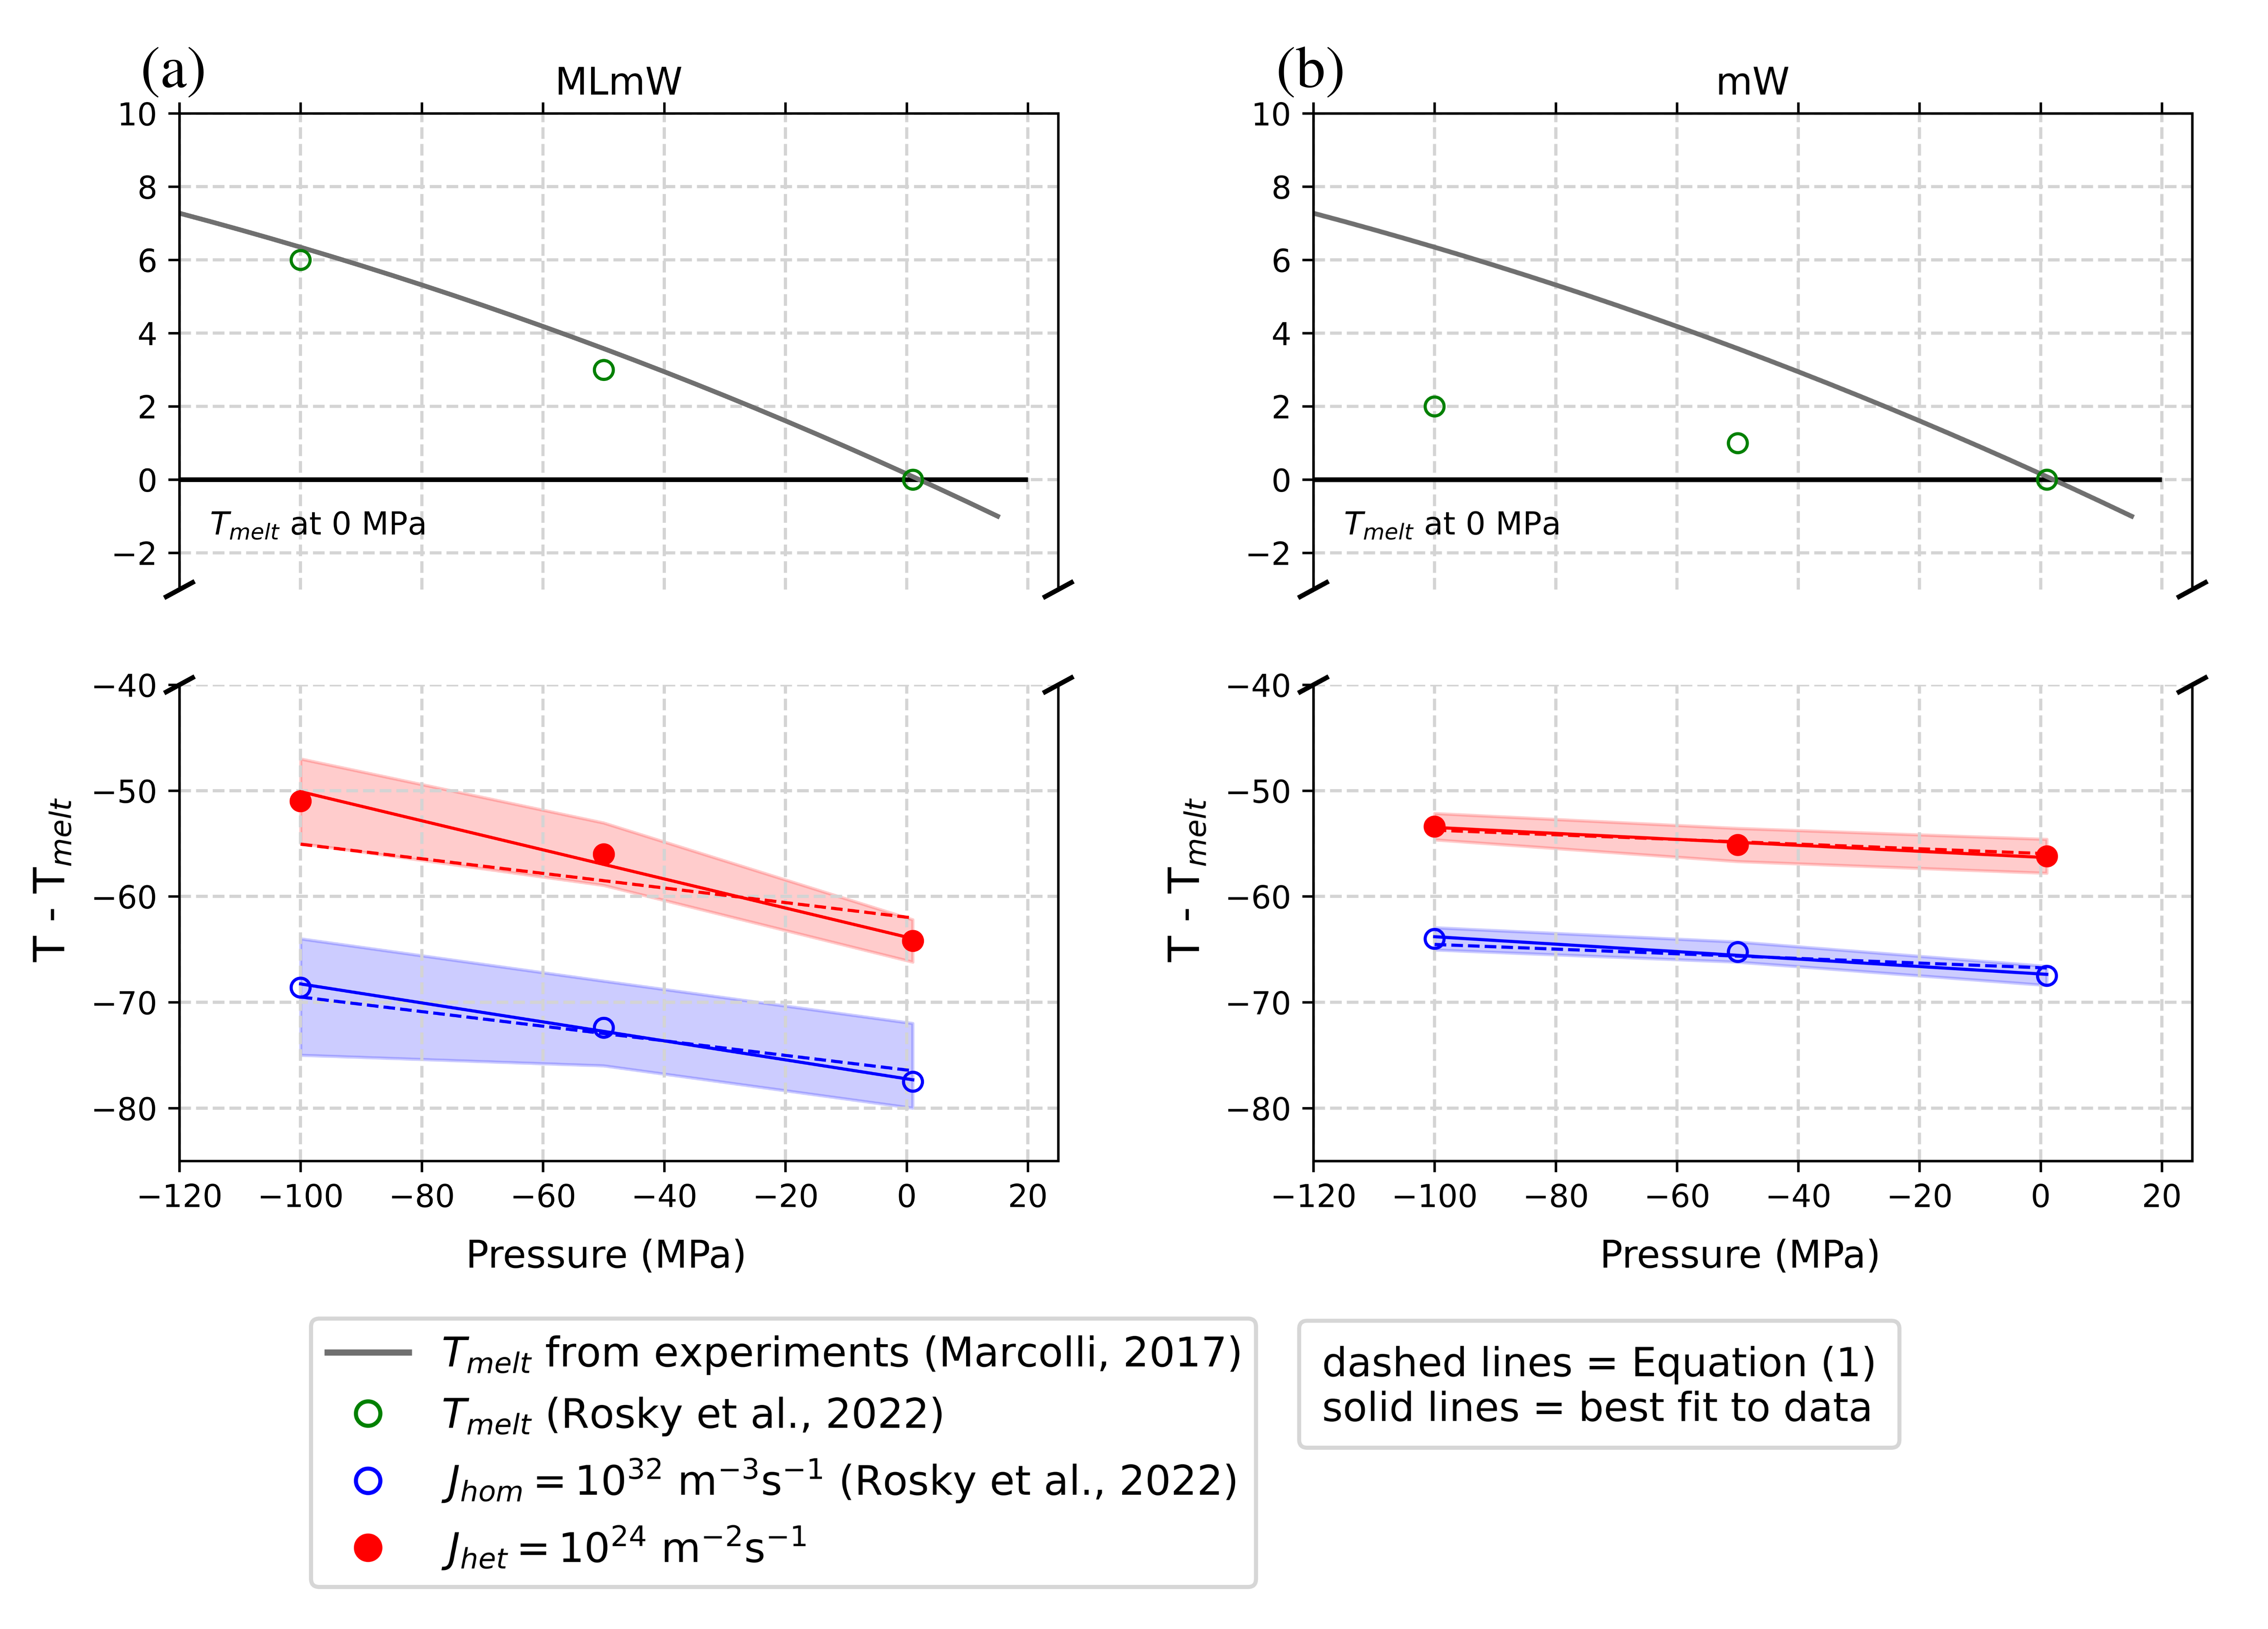
\includegraphics[width=12cm]{figures/homohet_PT_figure.png}
\caption{\label{fig:PT} Melting (green open circles), heterogeneous-freezing (red closed circles) and homogeneous freezing temperature (blue open circles) versus pressure. The heterogeneous freezing results are new, and the melting and homogeneous freezing results are reproduced from \citet{rosky2022} for comparison. The red and blue shading represents the 99\% confidence intervals (uncertainty) for the simulation data. Dashed lines use the slope predicted by Eq. (\ref{eq:dTdP}) to obtain a best fit to the intercept. Solid lines are a best linear fit of both slope and intercept. Contours of constant heterogeneous nucleation rate are, to within sampling uncertainty, linear and nearly parallel with lines of constant homogeneous nucleation rate for both the \DIFdelbeginFL \DIFdelFL{MLmW }\DIFdelendFL \DIFaddbeginFL \DIFaddFL{ML-mW }\DIFaddendFL model (a) and mW model (b).  The gray melting point line from \citet{marcolli2017} is a fit to experimental measurements, which the \DIFdelbeginFL \DIFdelFL{MLmW }\DIFdelendFL \DIFaddbeginFL \DIFaddFL{ML-mW }\DIFaddendFL model reproduces more realistically. Note that $-100$ MPa $= -1000$ atm.}
\end{figure*}


Freezing of water on \DIFdelbegin \DIFdel{a hydrophilic }\DIFdelend \DIFaddbegin \DIFadd{an ice-nucleating }\DIFaddend substrate (Fig. \ref{fig:configurations}(a)) is simulated at 1 atm, $-500$ atm and $-1000$ atm to identify how the intensive heterogeneous nucleation rate, $j_{het}$, behaves at negative pressures. The \DIFdelbegin \DIFdel{surface }\DIFdelend \DIFaddbegin \DIFadd{cooling rate and }\DIFaddend area of the substrate \DIFdelbegin \DIFdel{and the rate at which the system is cooled are two factors that determine the magnitude of $j_{het}$ that will be observed in these simulations, which in this case is $j_{het} = 10^{24}$ m$^{-2}$s$^{-1}$. Larger substrate area or slower cooling rate would each decrease the observed intensive heterogeneous nucleation rate. We keep these two factors }\DIFdelend \DIFaddbegin \DIFadd{in contact with water is kept }\DIFaddend fixed as we change the pressure of the system so that \DIFdelbegin \DIFdel{we observe the same magnitude }\DIFdelend \DIFaddbegin \DIFadd{the same magnitudes }\DIFaddend of $j_{het}$ \DIFaddbegin \DIFadd{is sampled }\DIFaddend at all pressures. For each pressure setting, we identify the temperature at which the intensive nucleation rate $j_{het}$ is equal to $10^{24}$ m$^{-2}$s$^{-1}$, thus obtaining contours of constant $j_{het}$ in pressure--temperature coordinates. Figure \ref{fig:PT} shows these results for both the \DIFdelbegin \DIFdel{MLmW }\DIFdelend \DIFaddbegin \DIFadd{ML-mW }\DIFaddend model and mW model. Intensive homogeneous nucleation rate data $j_{hom}$ (m$^{-3}$s$^{-1}$), as well as equilibrium melting points $T_m$ are also included in these plots for comparison \DIFdelbegin \DIFdel{from }\DIFdelend \DIFaddbegin \DIFadd{with }\DIFaddend \citet{rosky2022}. 

Comparing the data \DIFdelbegin \DIFdel{points for constant }\DIFdelend \DIFaddbegin \DIFadd{for }\DIFaddend intensive heterogeneous nucleation rate ($j_{het} = 10^{24}$ m$^{-2}$s$^{-1}$) with the data for \DIFdelbegin \DIFdel{constant }\DIFdelend intensive homogeneous nucleation rate ($j_{hom} = 10^{32}$ m$^{-3}$s$^{-1}$), we see that \DIFdelbegin \DIFdel{they follow a very }\DIFdelend \DIFaddbegin \DIFadd{the two follow a }\DIFaddend similar slope in pressure--temperature coordinates. Most significantly, we observe that the increase in temperature as a function of pressure for $j_{het}$ \DIFdelbegin \DIFdel{is linear to }\DIFdelend \DIFaddbegin \DIFadd{can be approximated as linear }\DIFaddend within the sampling uncertainty, indicating that the use of a linear \DIFdelbegin \DIFdel{approximation for $\Delta T/\Delta P$ is appropriate for }\DIFdelend \DIFaddbegin \DIFadd{estimate for $(\Delta T/\Delta P)_{het}$ may be applied to }\DIFaddend heterogeneous ice nucleation. For the mW model in particular, the slope predicted by Eq. (\ref{eq:dTdP}) fits exceptionally well to both the homogeneous and heterogeneous freezing data. Meanwhile, Eq. (\ref{eq:dTdP}) seems to \DIFdelbegin \DIFdel{slightly }\DIFdelend underestimate the heterogeneous slope of the \DIFdelbegin \DIFdel{MLmW model. Nevertheless}\DIFdelend \DIFaddbegin \DIFadd{ML-mW model. The source of excess steepness in the ML-mW heterogeneous slope is not uncovered in this study and merits further investigation. Despite this weakness}\DIFaddend , these results \DIFaddbegin \DIFadd{do }\DIFaddend indicate that the slope predicted by Eq. (\ref{eq:dTdP}) may still be applicable to heterogeneous nucleation, to within the simulation uncertainty. \DIFdelbegin \DIFdel{Thus we may conclude }\DIFdelend \DIFaddbegin \DIFadd{The similarity between the heterogeneous and homogeneous slopes for each respective water model suggest }\DIFaddend that $l_f$ and $\Delta v_{ls}$ remain key factors in determining the pressure dependence of heterogeneous nucleation rate. Indeed, \DIFdelbegin \DIFdel{it is significant to note that the observed slopes change consistently between mW and MLmW models , suggesting that the water density anomaly }\DIFdelend \DIFaddbegin \DIFadd{the consistent change in slope between the mW and ML-mW models indicate that the magnitude of density difference between liquid water and ice }\DIFaddend plays a similar \DIFdelbegin \DIFdel{key }\DIFdelend role for heterogeneous freezing as was previously found for homogeneous freezing \citep{rosky2022}.

In classical nucleation theory, $j_{het}$ has the form \citep{lamb2011physics}

\begin{equation} \label{eq:R}
    j_{het} = A\DIFaddbegin \DIFadd{_{het} }\DIFaddend \exp \! \left(\frac{C f_{het}}{T\Delta \mu ^2} \right),
\end{equation}

\noindent where $f_{het}$ is a heterogeneous compatibility function, typically related to the contact angle on the substrate, and $\Delta \mu$ is the chemical potential difference for the phase change. The factor $C = 16 \pi \gamma_{ls}^3 / (3 k_B \rho^2)$ depends on the liquid-solid surface tension ($\gamma_{ls}$) and density of ice ($\rho$). The \DIFaddbegin \DIFadd{pre-factor $A_{het}$ is related to the diffusivity of water molecules. The }\DIFaddend pressure dependence is introduced into this expression by using a formulation for chemical potential difference given by \citet{nemec2013}.
%Temperature dependent ice nucleation rate equation
%https://doi.org/10.1021/jp066080w
\DIFdelbegin \DIFdel{Equation (\ref{eq:dTdP}) is valid for heterogeneous, as well as homogeneous, ice nucleation, as long as the }\DIFdelend \DIFaddbegin \DIFadd{The }\DIFaddend heterogeneous compatibility function\DIFaddbegin \DIFadd{, }\DIFaddend $f_{het}$ of the substrate\DIFdelbegin \DIFdel{is not strongly pressure dependent, which has been }\DIFdelend \DIFaddbegin \DIFadd{, is }\DIFaddend formulated as a function of the effective contact angle between water and substrate \citep{lamb2011physics, zobrist2007}\DIFdelbegin \DIFdel{. The }\DIFdelend \DIFaddbegin \DIFadd{). As long as this term is not strongly pressure dependent; Equation (\ref{eq:dTdP}) is valid for heterogeneous, as well as homogeneous, ice nucleation. The roughly }\DIFaddend linear trend in our data suggest that the contact angle and compatibility function are not strongly dependent on pressure \DIFdelbegin \DIFdel{; this }\DIFdelend \DIFaddbegin \DIFadd{in the negative pressure regime studied here. This }\DIFaddend follows from the fact that the derivation of Eq. (\ref{eq:dTdP}) hinges on approximating many terms as constant along lines of constant $j$. If any of these assumptions are invalid \DIFaddbegin \DIFadd{in the negative pressure regime examined here}\DIFaddend , we would expect their effects to reveal themselves by producing a \DIFaddbegin \DIFadd{highly }\DIFaddend non-linear trend in pressure--temperature coordinates, which we do not observe. 

The \DIFaddbegin \DIFadd{thermodynamic }\DIFaddend values used in Eq. (\ref{eq:dTdP}) to produce the dashed lines \DIFdelbegin \DIFdel{in }\DIFdelend \DIFaddbegin \DIFadd{of }\DIFaddend Fig. \ref{fig:PT} are listed \DIFdelbegin \DIFdel{for each water model }\DIFdelend in Table \ref{tab:slopes} and \DIFdelbegin \DIFdel{are evaluated for }\DIFdelend \DIFaddbegin \DIFadd{correspond to }\DIFaddend bulk water (no proximity to an interface). As summarized in \DIFdelbegin \DIFdel{the table, using these values in Eq. (\ref{eq:dTdP}) predicts a slope }\DIFdelend \DIFaddbegin \DIFadd{column four of Table \ref{tab:slopes}, these values predict a slope of }\DIFaddend $\Delta T/\Delta P = -0.069$ K MPa$^{-1}$ for the \DIFdelbegin \DIFdel{MLmW model. When fitting a line to the heterogeneous data points from our simulations }\DIFdelend \DIFaddbegin \DIFadd{ML-mW model. A line of best fit to the simulated ML-mW heterogeneous freezing data gives instead a slope of $(\Delta T/\Delta P)_{het} = -0.14$ K MPa$^{-1}$ }\DIFaddend (solid red line in Fig. \ref{fig:PT}(a))\DIFdelbegin \DIFdel{, we instead find a slope of $-0.14$ K MPa$^{-1}$. The slope predicted by Eq. (\ref{eq:dTdP}) }\DIFdelend \DIFaddbegin \DIFadd{. The predicted slope }\DIFaddend (dashed red line in Fig. \ref{fig:PT}(a)) sits only marginally within the uncertainty bounds of the heterogeneous nucleation rate data and is 47\% steeper than \DIFdelbegin \DIFdel{our }\DIFdelend \DIFaddbegin \DIFadd{the }\DIFaddend best fit of the \DIFdelbegin \DIFdel{MLmW homogeneous freezing data }\DIFdelend \DIFaddbegin \DIFadd{homogeneous $(\Delta T/\Delta P)_{hom}$ data of the ML-mW model }\DIFaddend (See Table \ref{tab:slopes}).

We take some time to consider which factors may contribute to the steeper slope of heterogeneous freezing \DIFdelbegin \DIFdel{line of the MLmW }\DIFdelend \DIFaddbegin \DIFadd{in the ML-mW }\DIFaddend model compared to the homogeneous freezing line. \DIFdelbegin \DIFdel{Our hypothesis }\DIFdelend \DIFaddbegin \DIFadd{One hypothesis is }\DIFaddend that Eq. (\ref{eq:dTdP}) still holds \DIFaddbegin \DIFadd{true }\DIFaddend for heterogeneous ice nucleation, but that adjustments need to be made to the values of $\Delta v_{ls}$ or $l_f$ used in the equation \DIFdelbegin \DIFdel{. While the linear nature of $(\Delta T/\Delta P)$ is apparent in our results}\DIFdelend \DIFaddbegin \DIFadd{to achieve quantitative agreement with the heterogeneous freezing line. While our results support that the trend in $(\Delta T/\Delta P)_{het}$ can be approximated as linear in the negative pressure regime}\DIFaddend , we are less confident in the quantitative values of $\Delta v_{ls}$ and $l_f$ for heterogeneous freezing compared to homogeneous freezing. In the homogeneous case, the values of $T_m$, $l_f$, and $\Delta v_{ls}$ are well constrained because they can be calculated from bulk water, \DIFdelbegin \DIFdel{and as a result we see }\DIFdelend \DIFaddbegin \DIFadd{which could account for the }\DIFaddend excellent agreement between Eq. (\ref{eq:dTdP}) and the homogeneous simulation results of \citet{rosky2022}. For the heterogeneous case, there is more ambiguity around these thermodynamic values because the properties of water near an interface may differ from the bulk properties. We see that by using \DIFdelbegin \DIFdel{the }\DIFdelend bulk thermodynamic values in Eq. (\ref{eq:dTdP}), we underestimate the slope \DIFaddbegin \DIFadd{of $(\Delta T/\Delta P)_{het}$ }\DIFaddend by up to 50\%. Interestingly, this \DIFdelbegin \DIFdel{difference in }\DIFdelend \DIFaddbegin \DIFadd{discrepancy between the }\DIFaddend homogeneous and heterogeneous slopes is seen only \DIFdelbegin \DIFdel{with the MLmW }\DIFdelend \DIFaddbegin \DIFadd{in the ML-mW }\DIFaddend model. Meanwhile the homogeneous and heterogeneous freezing lines are nearly parallel for the mW model. This could indicate the thermodynamic properties of mW water are less influenced near the substrate compared to the \DIFdelbegin \DIFdel{MLmW model. }\DIFdelend \DIFaddbegin \DIFadd{ML-mW model. This interpretation is supported by \mbox{%DIFAUXCMD
\citet{qiu2018graphiteinterface} }\hspace{0pt}%DIFAUXCMD
which identified mW water at the mW-Carbon interface as having thermodynamics similar to that of the bulk liquid.
}

\DIFadd{Another possibility is that the contact angle and surface free energy (surface tension) between water and substrate exerts an influence on the slope of $(\Delta T/\Delta P)_{het}$. We are not aware of any experimental evidence to support that the heterogeneous and homogeneous freezing lines are parallel in P--T coordinates. \mbox{%DIFAUXCMD
\citet{evans1967} }\hspace{0pt}%DIFAUXCMD
showed that a heterogeneous freezing line for aqueous suspension of ice-nucleating material at positive pressures is actually less steep than the melting point line, and thus also less steep than the homogeneous line. Although the mW-substrate and ML-mW--substrate were designed to exhibit the same freezing temperature enhancements over the homogeneous freezing temperature, they do have different contact angles between the water and substrate. Thus, this could potentially be a factor involved in the discrepancy between ML-mW homogeneous and heterogeneous slopes compares to the mW case where the two lines are parallel.
}\DIFaddend 

In \DIFdelbegin \DIFdel{all cases}\DIFdelend \DIFaddbegin \DIFadd{our simulation results}\DIFaddend , using bulk water thermodynamic values in Eq. (\ref{eq:dTdP}) provides a lower-bound to the slope of \DIFdelbegin \DIFdel{$(\Delta T/\Delta P)$}\DIFdelend \DIFaddbegin \DIFadd{$(\Delta T/\Delta P)_{het}$}\DIFaddend , which can be very useful in estimating the increase in heterogeneous freezing temperature due to negative pressure \DIFaddbegin \DIFadd{in atmospheric and experimental contexts}\DIFaddend . However, further investigation is needed to identify a robust way to \DIFdelbegin \DIFdel{obtain values $l_f$, $\Delta v_{ls}$ that will }\DIFdelend account for the observed steepness of the \DIFdelbegin \DIFdel{MLmW }\DIFdelend \DIFaddbegin \DIFadd{ML-mW }\DIFaddend heterogeneous nucleation slope. Going forward, the linearity and the theoretical prediction of the slope are probably adequate for practical use, given other significant uncertainties in using classical nucleation theory. 



\begin{table}
\DIFaddbeginFL \caption{\label{tab:slopes} \DIFaddFL{Parameters entering Eq. (\ref{eq:dTdP}) for homogeneous and heterogeneous nucleation, for both mW and ML-mW models. Dashes indicate that a measurement of this value is not known to us. Sources: $^a$ \mbox{%DIFAUXCMD
\citet{chan2019}}\hspace{0pt}%DIFAUXCMD
, $^b$ \mbox{%DIFAUXCMD
\citet{rosky2022}}\hspace{0pt}%DIFAUXCMD
.}}
\DIFaddendFL \begin{tabular}{ |p{2.60cm}||p{2.2cm}|p{2.2cm}|p{2.2cm}|p{2.2cm}|p{2.5cm}|  }
 \hline
 & \multicolumn{1}{|c|}{$l_f$}  
 & \multicolumn{1}{|c|}{$T_m$}
 & \multicolumn{1}{|c|}{$\Delta v_{ls}$}
 & \multicolumn{1}{|c|}{$\frac{T_m \Delta v_{ls}}{l_f}$ } 
 & \multicolumn{1}{|c|}{$\Delta T/ \Delta P$ best fit }\\
 & \multicolumn{1}{|c|}{[J/mol] }  
 & \multicolumn{1}{|c|}{[K] }
 & \multicolumn{1}{|c|}{[m$^3$/mol]  }        
 & \multicolumn{1}{|c|}{[K/MPa] }                           
 & \multicolumn{1}{|c|}{[K/MPa] }\\
 \hline
 mW $J_{hom}$   & 5271.8 $^a$           & 273 $^{a,b}$  &  $-4.2 \times 10^{-7}$ $^{a,b}$     & $-0.022$    & $-0.035$ \\
 mW $J_{het}$   & - - -   & 273           & - - -   &           & $-0.028$ \\
 \DIFdelbeginFL \DIFdelFL{MLmW }\DIFdelendFL \DIFaddbeginFL \DIFaddFL{ML-mW }\DIFaddendFL $J_{hom}$ & 5857.6 $^a$           & 292 $^b$      & $-13.8 \times 10^{-7}$ $^{a,b}$     & $-0.069$    & $-0.089$ \\
 \DIFdelbeginFL \DIFdelFL{MLmW }\DIFdelendFL \DIFaddbeginFL \DIFaddFL{ML-mW }\DIFaddendFL $J_{het}$ & - - -   & 292           & - - -   &           & $-0.14$ \\
 Real water $J_{hom}$ & 6025.0 $^a$     & 273.15 $^a$   & $-16.1 \times 10^{-7}$ $^{b}$       & $-0.073$    & - - - \\
 \hline
\end{tabular}
\DIFdelbeginFL %DIFDELCMD < \caption{%
{%DIFAUXCMD
%DIFDELCMD < \label{tab:slopes} %%%
\DIFdelFL{Parameters entering Eq. (\ref{eq:dTdP}) for homogeneous and heterogeneous nucleation, for both mW and MLmW models. Dashes indicate that a measurement of this value is not known to us. Sources: $^a$ \mbox{%DIFAUXCMD
\citet{chan2019}}\hspace{0pt}%DIFAUXCMD
, $^b$ \mbox{%DIFAUXCMD
\citet{rosky2022}}\hspace{0pt}%DIFAUXCMD
.}}
%DIFAUXCMD
\DIFdelendFL \end{table}




\subsection{Heterogeneous ice nucleation in water capillary bridges} \label{capillary}

One way for water to exist stably under negative pressure is through geometric configurations which produce high degrees of negative surface curvature at the air-water interface, such as inside a water capillary bridge. The negative pressure experienced by the water in these cases is a result of Laplace pressure, $P = \sigma_{lv}(\frac{1}{r_1}+\frac{1}{r_2})$, where $\sigma_{lv}$ is the surface tension between liquid and vapor, and $r_1$ and $r_2$ are the radii of curvature of the air-water interface. In these cases, the equilibrium pressure within the water is smaller than the external environmental pressure, allowing for negative pressure to exist within water that is otherwise in a 1 atm environment. The Laplace pressure associated with different capillary geometries is summarized by \citet{elliott2021}. For the capillary bridge configuration used in this study, shown in Fig. \ref{fig:configurations}(c), the expected Laplace pressure within the water is

\begin{equation} \label{eq:dPh}
   \Delta P = -\sigma_{lv} \frac{2\cos(\theta)}{h},
\end{equation}

\noindent where $\theta$ is the contact angle between water and the substrate. By substituting the above equation into Eq. (\ref{eq:dTdP}), we obtain an expression to predict the temperature increase for a given nucleation rate $j_{het}$ as a function of inverse capillary bridge height,  

\begin{equation}\label{eq:dTh}
     \Delta T = -2 \sigma_{lv}\cos(\theta) \frac{\Delta \nu_{ls} T_m }{l_f} \left(\frac{1}{h}\right).
\end{equation}

\noindent Given the previous conclusion that terms $\sigma_{lv}$ and $\theta$ do not change significantly with pressure, we expect a linear relationship between freezing temperature and inverse capillary height $1/h$. Figure \ref{fig:capillary} shows the freezing temperatures corresponding to an intensive heterogeneous nucleation rate $j_{het} = 10^{24}$ m$^{-2}$s$^{-1}$ inside water capillary bridges with heights $h = 30$, $24$, and $18$ \AA{}. We find that the data follows a linear trend as anticipated. As will be discussed in Sec. \ref{ice locations}, we have excluded the 18 \AA{} capillary bridge from the current analysis because this scale of confinement of the water between the substrate surfaces causes an increase in ice nucleation rate that cannot be attributed to negative pressure alone.

\begin{figure}[t]
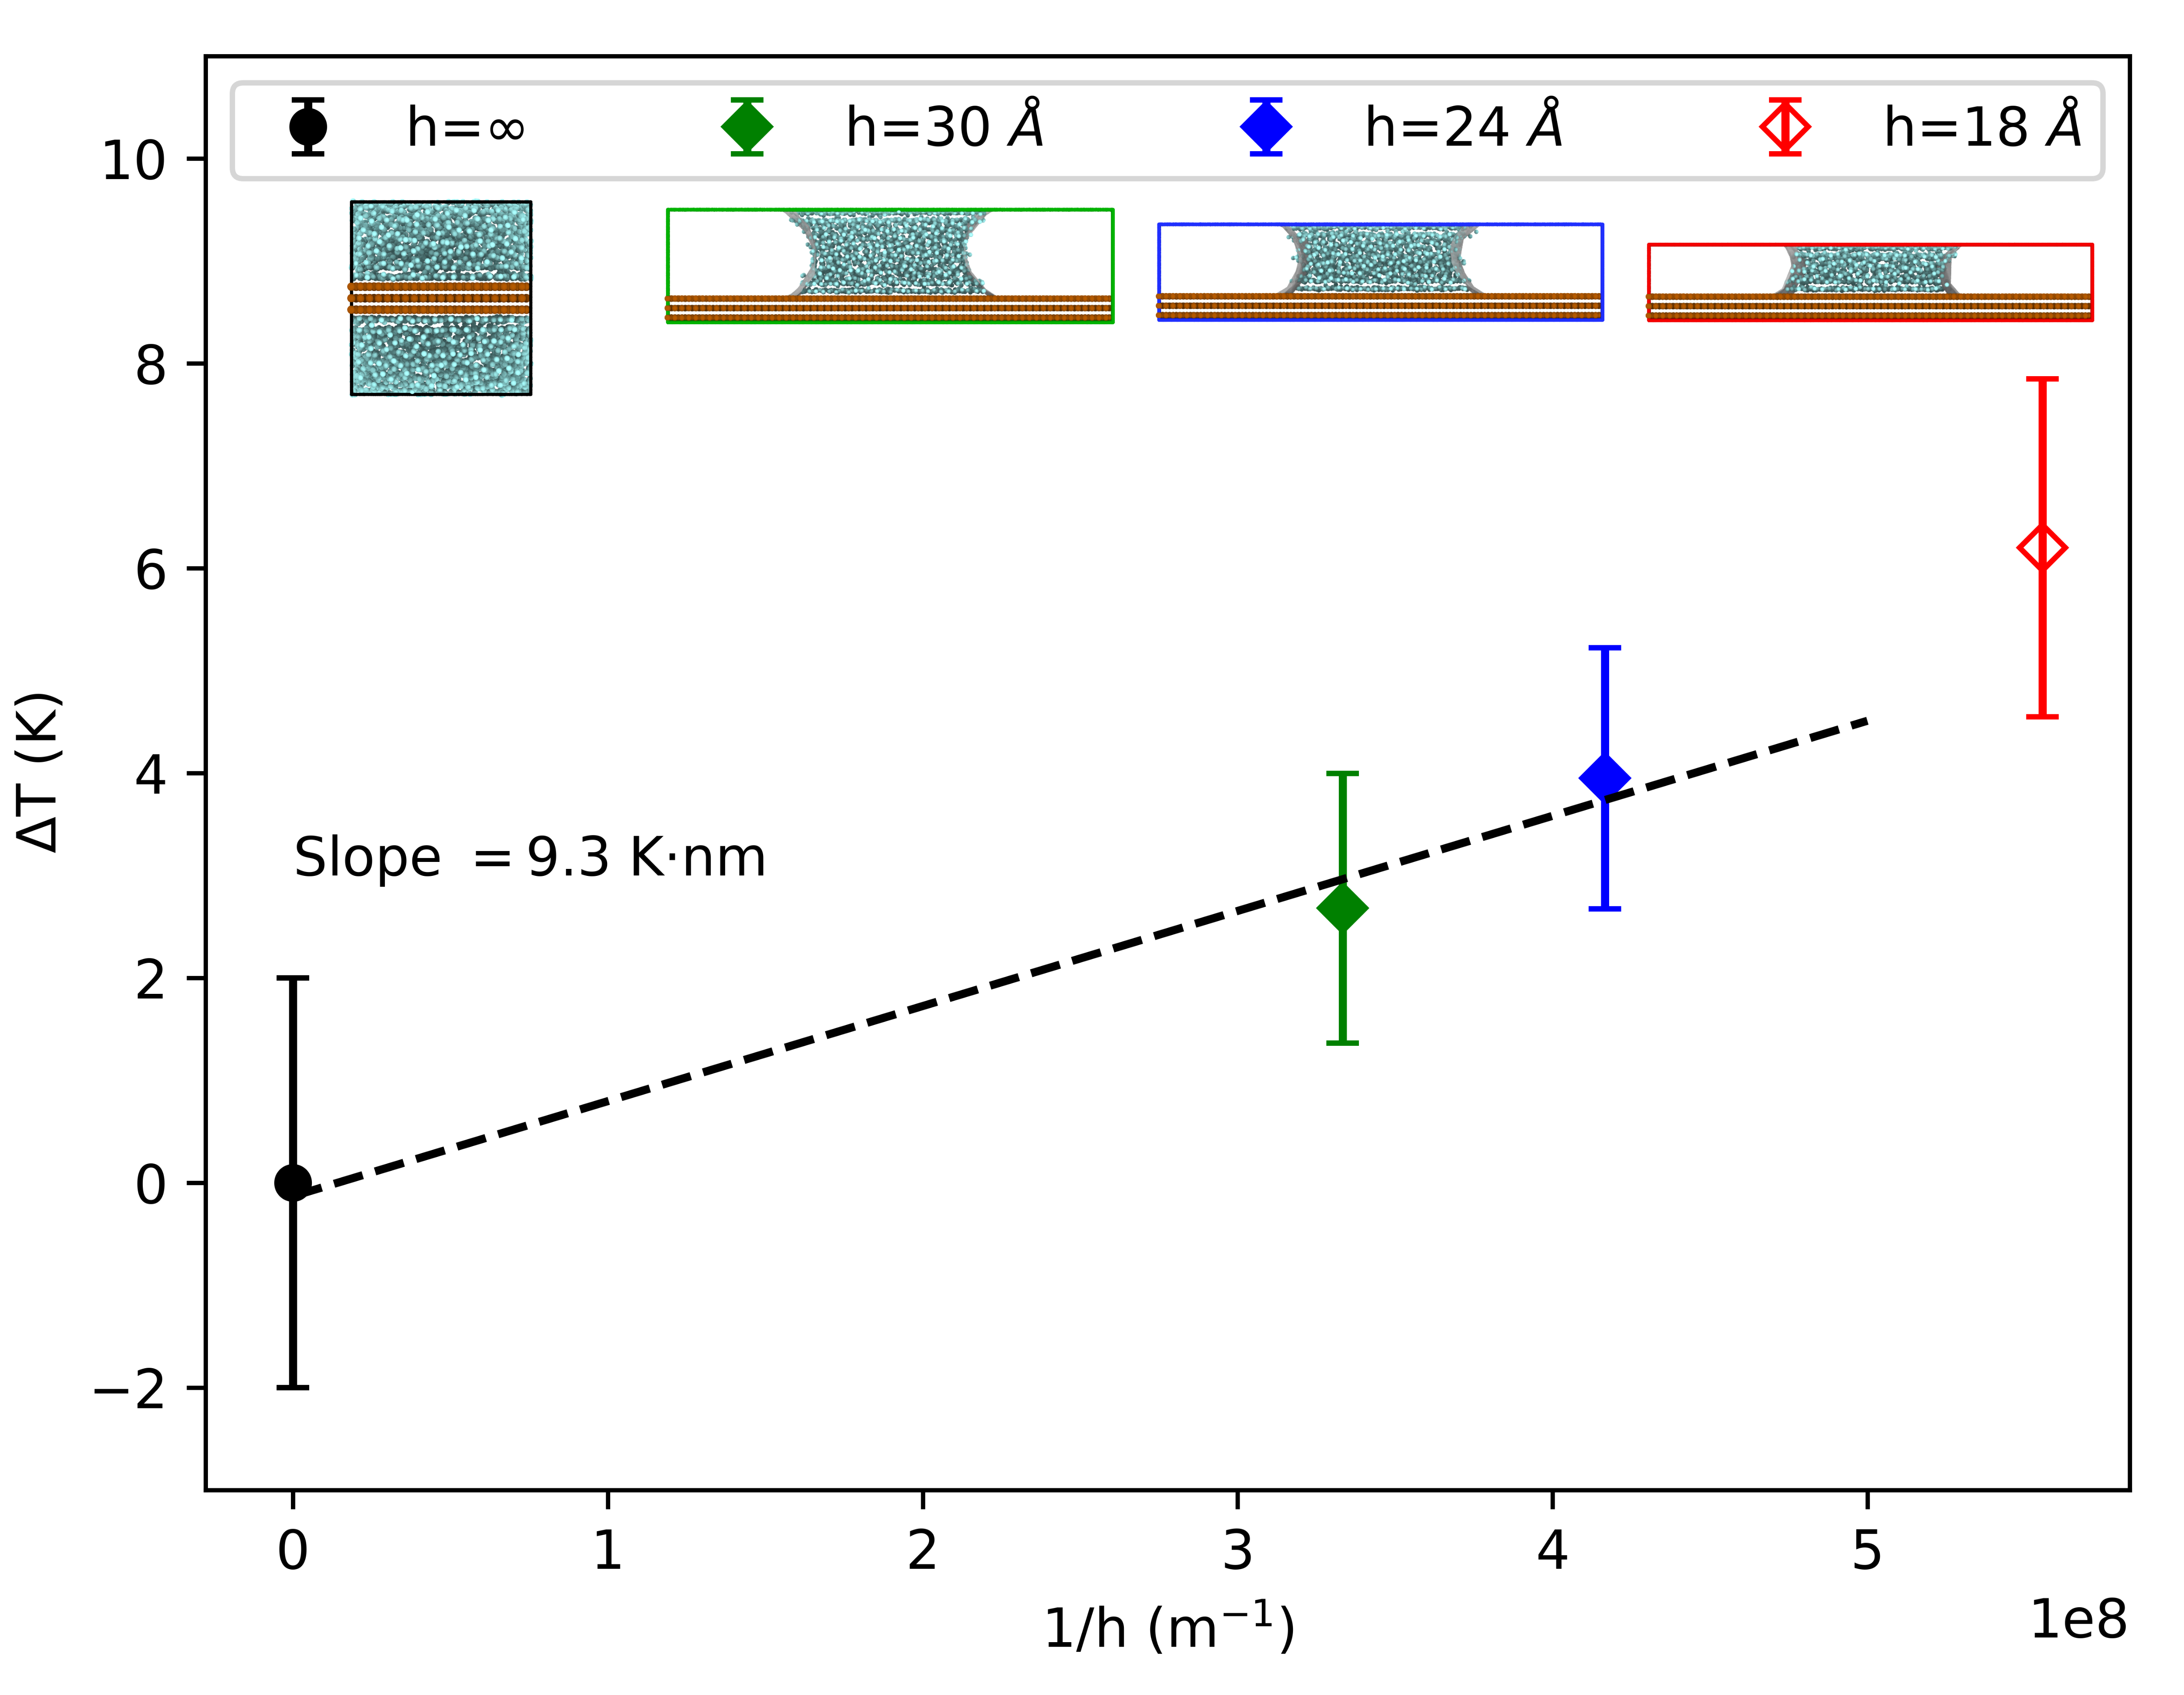
\includegraphics[width=8.3cm]{figures/TvH_inset.png}
\caption{Increase in heterogeneous freezing temperature $\Delta T$ versus $1/h$ for capillary-bridge heights of $h = 30$ (green filled diamond), 24 (blue filled diamond), and 18 \AA{} (red open diamond), as well as for bulk water (filled black circle) in contact with identical \DIFdelbeginFL \DIFdelFL{hydrophilic }\DIFdelendFL \DIFaddbeginFL \DIFaddFL{ice-nucleating }\DIFaddendFL substrates. Excluding the 18-\AA{} capillary (red diamond) which is influenced by confinement effects, the line of constant nucleation rate as a function of inverse capillary height follows a linear trend \DIFaddbeginFL \DIFaddFL{shown by the linear best fit to the data (dashed black line)}\DIFaddendFL . The 18-\AA{} capillary data is not included in the linear fit to obtain the indicated slope $\Delta T \cdot h$.}
    \label{fig:capillary}
\end{figure}


%DIF < Calculating approximate negative pressure induced using capillary equation (Elliott), using surface tension that is given by Molinero and verified for MLmW via my own calculations.
%DIF > Calculating approximate negative pressure induced using capillary equation (Elliott), using surface tension that is given by Molinero and verified for ML-mW via my own calculations.

%Negative Laplace pressure results in an increasing nucleation temperature, consistent with Equation . As expected from the confinement effects at scales less than 24 A, the 18 A capillary bridge deviates from the linear trend that would be attributed to Laplace pressure effects alone. 

We can now use the linear slope $-2 \sigma_{lv}\cos(\theta) \left[\frac{\Delta \nu_{ls} T_m }{l_f}\right]$ from Eq. (\ref{eq:dTh}) to analyze the results in Fig. \ref{fig:capillary}. A linear fit to the data points \DIFaddbegin \DIFadd{shown by the dashed black line }\DIFaddend in Fig. \ref{fig:capillary} produces a slope $(\Delta T \cdot h)$ of $9.3$ K$\cdot$m. We also know from our analysis of $(\Delta T/\Delta P)$ in Sec. \ref{sec:hetrate} and Table \ref{tab:slopes} that the best fit value of $\left[\frac{\Delta \nu_{ls} T_m }{l_f}\right]$ for the \DIFdelbegin \DIFdel{MLmW }\DIFdelend \DIFaddbegin \DIFadd{ML-mW }\DIFaddend model is $-0.14$ K MPa$^{-1}$. We substitute these two slopes into Eq. (\ref{eq:dTh}) to solve for the value $\sigma_{ls} cos(\theta) = 0.042$ J m$^{-2}$. The surface tension $\sigma_{ls}$ of the mW model was reported by \citet{molinero2009} to be $0.066$ J m$^{-2}$, and by following methods of \citet{li2009surface} (supplementary material), we found the same value for the \DIFdelbegin \DIFdel{MLmW }\DIFdelend \DIFaddbegin \DIFadd{ML-mW }\DIFaddend model. Using this value of $\sigma_{ls}$, we solve for the contact angle $\theta = 50.5$ degrees. This value of $\theta$ is consistent with estimates we obtain by measuring the radius of curvature of the capillary bridge air-water interfaces using a method similar to \citet{giovambattista2007}. With these estimates of $\sigma_{ls}$ and $\theta$, we can also use Eq. (\ref{eq:dPh}) to calculate the magnitude of Laplace pressure that may be present within the water capillary bridges. The 24-\AA{} capillary bridge has a pressure of $-345$ atm, and the 30-\AA{} bridge a pressure of $-275$ atm.

Our main findings are that negative Laplace pressure created within water capillary bridges increases the temperature of $j_{het}$ in a manner that is consistent with the linear slope of $\Delta T/\Delta P$ combined with the expected Laplace pressure for this capillary geometry. A 24-\AA{} capillary bridge can exhibit a $\approx 3$-K increase in heterogeneous freezing temperature, and a $\approx 2$-K increase within a 30-\AA{} water capillary bridge.

\subsection{Effect of confinement between substrate layers}
\DIFdelbegin \DIFdel{The }\DIFdelend \DIFaddbegin \DIFadd{Capillary theory is expected to remain valid at the nano-scale \mbox{%DIFAUXCMD
\citep{elliott2021}}\hspace{0pt}%DIFAUXCMD
, however the }\DIFaddend ice nucleation rate in water can be effected by confined geometries \DIFdelbegin \DIFdel{\mbox{%DIFAUXCMD
\citep{cao2019, roudsari2022}}\hspace{0pt}%DIFAUXCMD
}\DIFdelend \DIFaddbegin \DIFadd{\mbox{%DIFAUXCMD
\citep{cao2019, roudsari2022, hussain2021contactfreezing}}\hspace{0pt}%DIFAUXCMD
}\DIFaddend . When analyzing the increase in freezing temperature within the water capillary bridges, we need to disentangle the effects of confinement from the effects of Laplace pressure. To do so, we ran simulations to observe how confinement alone affects ice nucleation rate on the substrate. We use the configuration shown in Fig. \ref{fig:configurations}(b), where the spacing between the substrate surfaces along the $z$-axis dimension has been reduced to 18, 24 and 30 \AA{} to match the levels of confinement present in our water capillary bridges. In these simulations, water molecules are confined between the substrate surfaces, but \DIFdelbegin \DIFdel{do not have the }\DIFdelend \DIFaddbegin \DIFadd{have no }\DIFaddend air-water interface that gives rise to Laplace pressure. \DIFaddbegin \DIFadd{The pressure in the boxes is set to 1 , $-500$, and $-1000$ atm, to directly compare against the ``unconfined'' configuration across the full range of pressures. }\DIFaddend Results are plotted in Fig. \ref{fig:confinement}(a), showing that 24 and 30-\AA{} separations (blue and green data points) have identical freezing temperatures at all pressures as the ``unconfined'' configuration (black data points). This allows us to conclude that the \DIFdelbegin \DIFdel{trends }\DIFdelend \DIFaddbegin \DIFadd{freezing temperature enhancement }\DIFaddend reported previously, e.g. for 24 and 30-\AA{} capillary bridges in Fig. \ref{fig:capillary}, are due to pressure alone. The 18-\AA{} setup (red data points in Fig. \ref{fig:confinement}(a)) exhibits a significant increase in freezing temperature as a result of the confined geometry. This behavior is indeed evident in the \DIFaddbegin \DIFadd{departure of the }\DIFaddend 18-\AA{} capillary bridge freezing data \DIFaddbegin \DIFadd{point from the linear trend }\DIFaddend in Fig. \ref{fig:capillary}\DIFdelbegin \DIFdel{, which }\DIFdelend \DIFaddbegin \DIFadd{. This }\DIFaddend is why we have excluded the 18-\AA{} capillary bridge data from the slope analysis in the previous section.
\DIFdelbegin \DIFdel{Other research \mbox{%DIFAUXCMD
\citep{elliott2021} }\hspace{0pt}%DIFAUXCMD
supports that capillary theory can extend to the nano-scale used in our simulations, which our results corroborate. Meanwhile, our results are also consistent with \mbox{%DIFAUXCMD
\citet{Almeida2021}}\hspace{0pt}%DIFAUXCMD
, who indicate that the capillary theory breaks down with separations less than $\approx 20$ \AA{}.
}\DIFdelend 

\begin{figure*}[t]
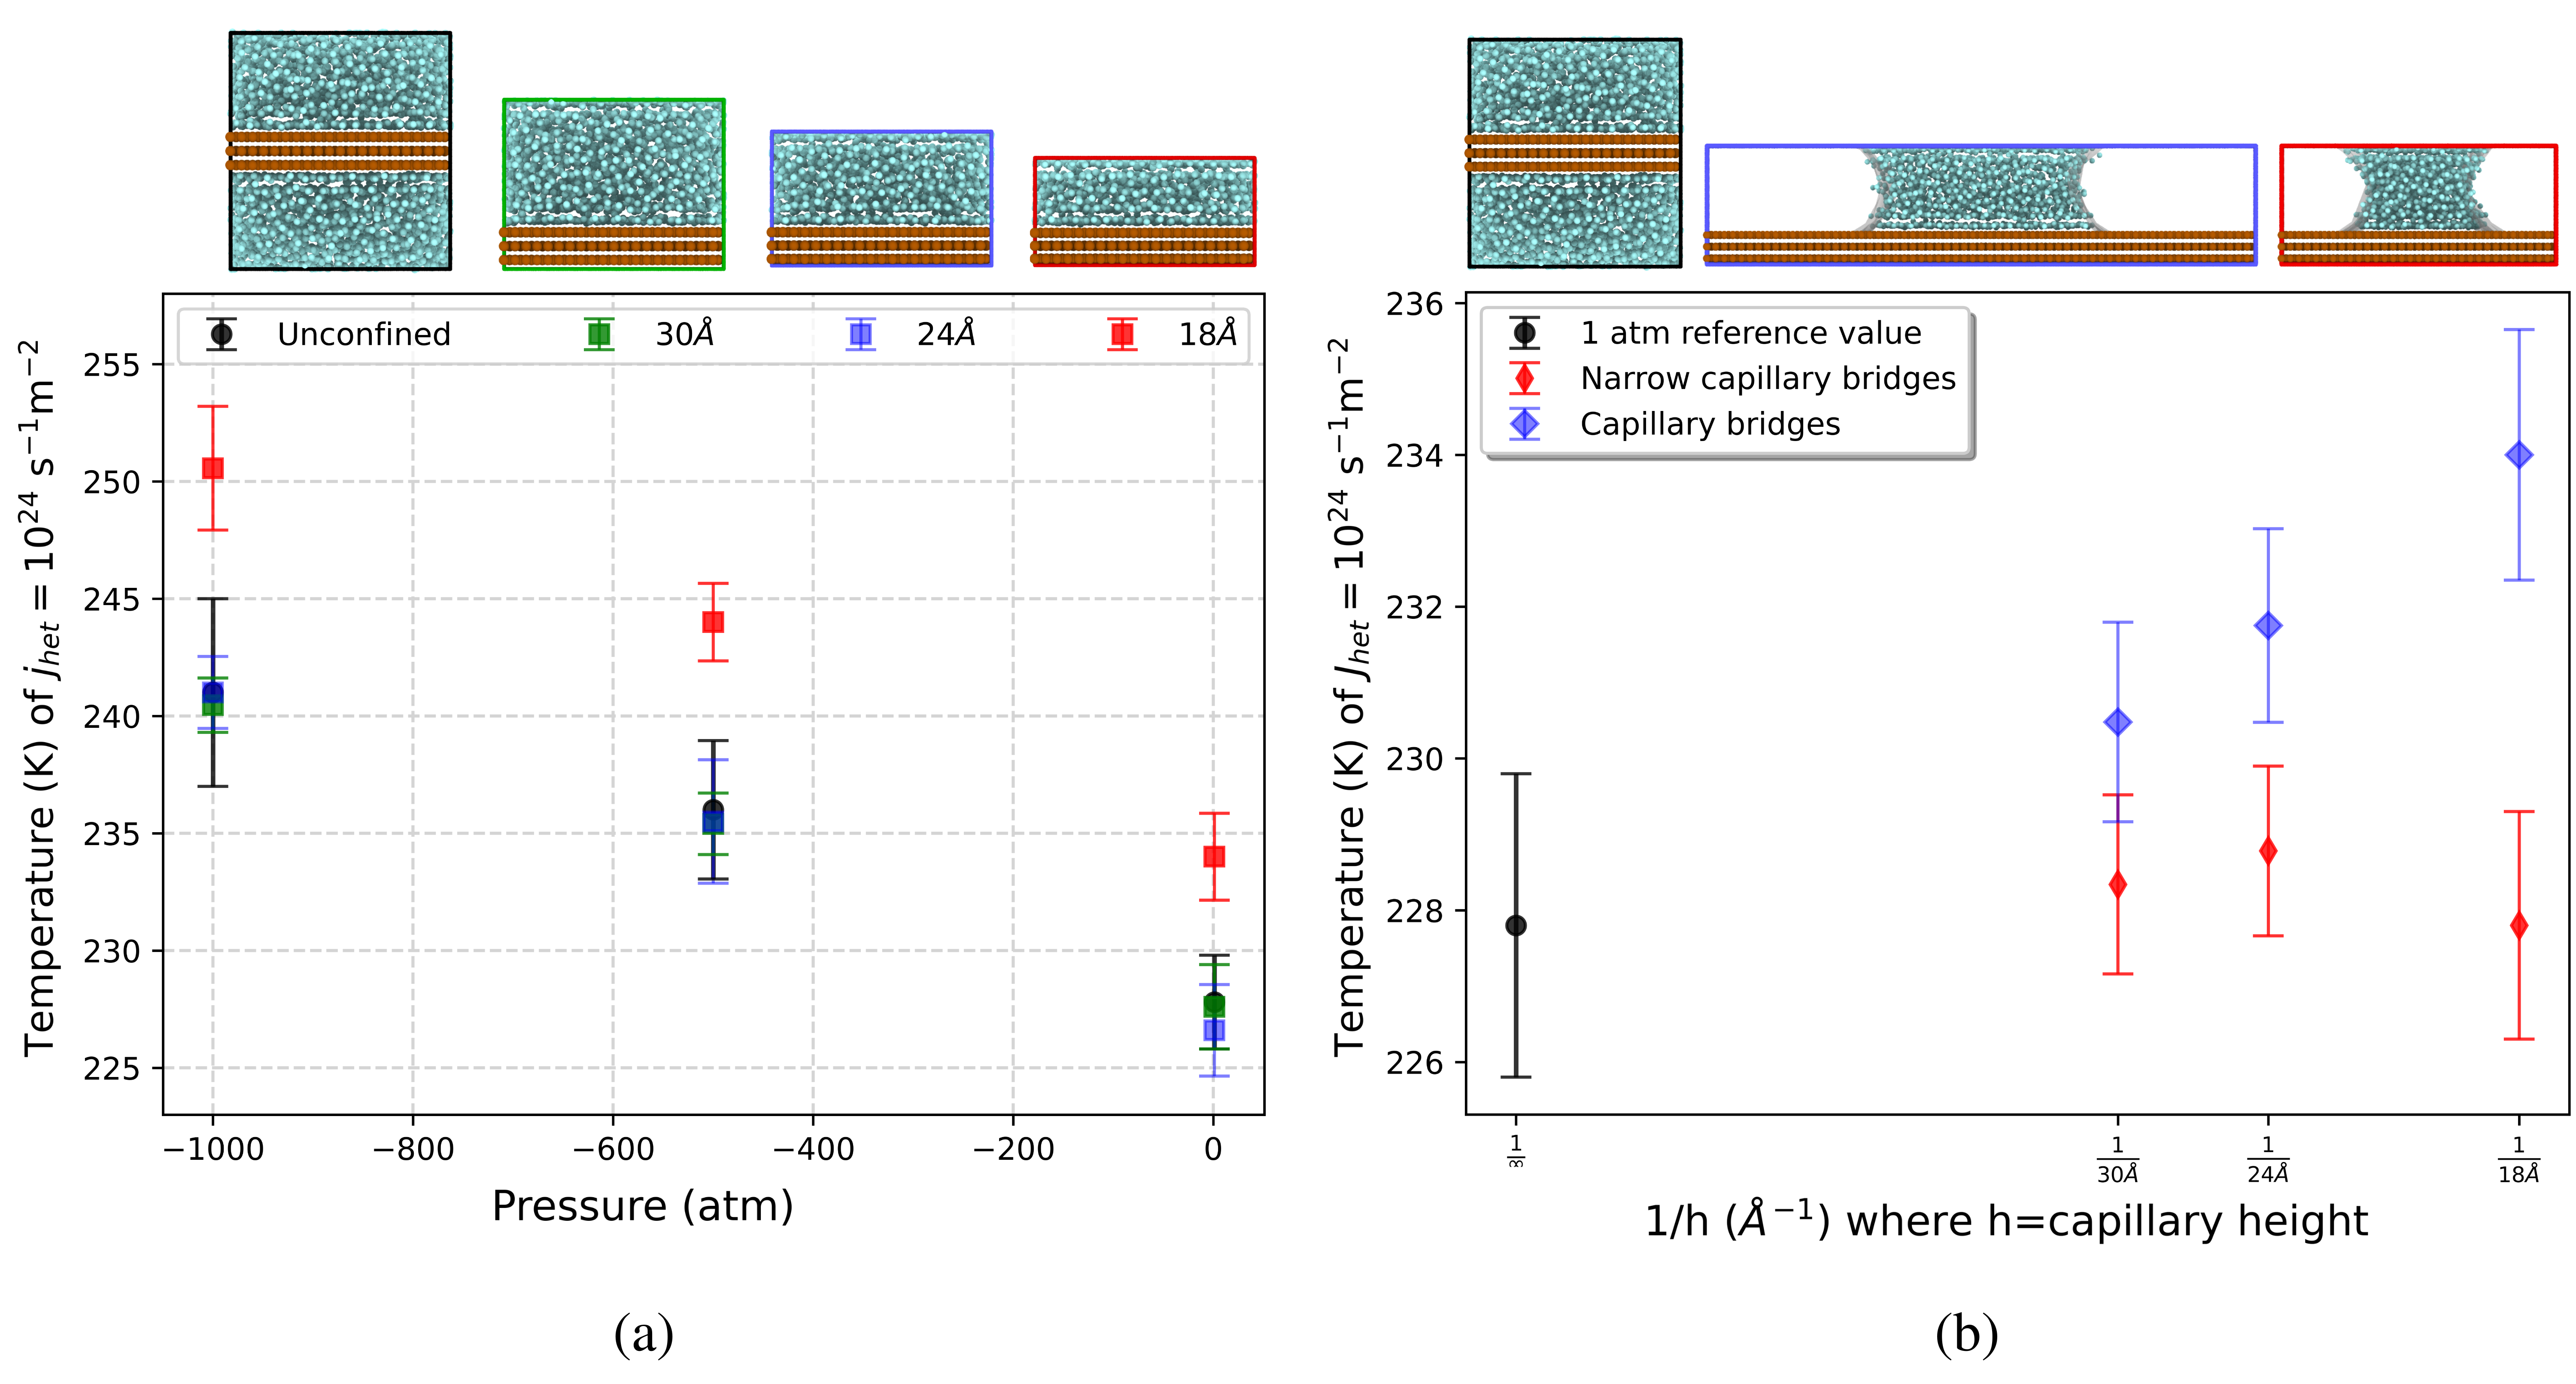
\includegraphics[width=12cm]{figures/confinement_effects.png}
\caption{(a) Heterogeneous freezing temperature versus pressure with varying separation between substrates, illustrating the effect of confinement along the $z$-axis. We see that confinement influences the ice nucleation rate for only the 18-\AA{} configuration (red squares). The 24-\AA{} (blue squares) and 30-\AA{} (green squares) confinement configurations exhibit the same freezing temperatures at all pressures as the ``unconfined'' reference simulations (black circles). (b) Heterogeneous freezing temperature versus inverse capillary-bridge height for varying widths of the capillary bridge, showing the effect of confinement along the $x$-axis between air-water interfaces. Confining the water within a narrow capillary bridge (red diamonds) suppresses the increase in freezing temperature that is seen in the capillary bridges that are twice as wide (blue diamonds).}
\label{fig:confinement}
\end{figure*}



\subsection{Freezing locations relative to the air-water interface} \label{ice locations}

We now consider whether there is an analogous confinement effect along the $x$-axis, between the two air-water interfaces of our capillary bridge simulations. \DIFaddbegin \DIFadd{A narrow capillary bridge configuration can be seen in Fig. \ref{fig:configurations}(d), where the total surface area of substrate-water contact is kept constant by doubling the $y$-dimension of the simulation box while halving the width of the capillary bridge. The narrow capillary bridges are 30 \AA{} wide, while the capillary bridges used in our previous results (henceforth referred to as ``wide capillary bridges'') are 60 \AA{} wide. The reported width of the capillary bridges is measured at the water--substrate interface. Figure \ref{fig:confinement}(b) shows heterogeneous freezing rate temperature as a function of $1/h$ for the wide capillary bridges (blue diamonds), compared with narrow capillary bridges (red diamonds). We observe that confining the water within a narrow capillary bridge eliminates the temperature enhancement from Laplace pressure that is observed in the wide capillaries. We attribute this effect to an apparent suppression of ice nucleation near the air-water interface, as discussed below. 
}

\DIFaddend Figure \ref{fig:freezinglocations}(a) shows the \DIFaddbegin \DIFadd{$x,z$-plane }\DIFaddend locations of ice nucleation events \DIFdelbegin \DIFdel{throughout a capillary bridges }\DIFdelend \DIFaddbegin \DIFadd{within the 60 \AA{} wide, 30 \AA{} tall capillary bridge }\DIFaddend viewed from the side\DIFdelbegin \DIFdel{, with the }\DIFdelend \DIFaddbegin \DIFadd{. The }\DIFaddend air-water interface \DIFaddbegin \DIFadd{is }\DIFaddend shown in red shading. Figure \ref{fig:freezinglocations}(b) shows the \DIFdelbegin \DIFdel{ice nucleation locations }\DIFdelend \DIFaddbegin \DIFadd{combined locations of ice nucleation events in the 24 \AA{} and 30 \AA{} tall capillary bridges, as viewed from above }\DIFaddend in the $x,y$-plane\DIFdelbegin \DIFdel{, viewing the capillary bridge from above}\DIFdelend \DIFaddbegin \DIFadd{. In this case, the red shading indicates the position of the air-water interface in contact with the substrate}\DIFaddend . We see that nucleation is preferred near the substrate as expected, but also that it is suppressed near the air-water interfaces. In Fig. \ref{fig:freezinglocations}(c) we plot freezing \DIFdelbegin \DIFdel{locations }\DIFdelend \DIFaddbegin \DIFadd{probability density }\DIFaddend as a function of distance from the nearest substrate surface \DIFaddbegin \DIFadd{using all freezing events in the 24 \AA{} and 30 \AA{} tall capillary bridges}\DIFaddend . Because this distribution is asymmetric (being affected by the substrate on one side) we fit a gamma distribution to the data to find that 99\% of nucleation events occur at distances between 3.2 and 6.9 \AA{} from the substrate, along the $z$-axis. Figure \ref{fig:freezinglocations}(d) shows the probability \DIFdelbegin \DIFdel{distribution }\DIFdelend \DIFaddbegin \DIFadd{density }\DIFaddend of ice nucleation as a function of distance from the nearest air-water interface \DIFaddbegin \DIFadd{using all freezing events in the 24 \AA{} and 30 \AA{} capillary bridges}\DIFaddend . Analyzing this spatial distribution of ice nucleation events, we observe that ice nucleation never occurs within \DIFaddbegin \DIFadd{approximately }\DIFaddend 10 \AA{} of the air-water interface. \DIFdelbegin \DIFdel{Additionally, there is a statistically significant preference for ice nucleation to occur between 20 and 25 \AA{} from the air-water interface. Thus, it appears that ice nucleation has a preference for the }\DIFdelend \DIFaddbegin \DIFadd{This lack of heterogeneous ice nucleation in the immediate vicinity of air--water interface could be related to premelting at the ice--vapor interface, described for the mW model by \mbox{%DIFAUXCMD
\citet{qiu2018premelting}}\hspace{0pt}%DIFAUXCMD
.
}

\DIFadd{The narrow capillary bridges being 30 \AA{} wide implies that most of the water molecules are positioned within the 10-\AA{} regions near the }\DIFaddend air-water interface \DIFdelbegin \DIFdel{but avoids immediate proximity}\DIFdelend \DIFaddbegin \DIFadd{where no ice nucleation events are observed. In all of the narrow bridge heights (red diamonds in \ref{fig:confinement}(b)) the heterogeneous freezing temperature is the same as the 1 atm reference temperature (black data point in Fig. \ref{fig:confinement}(b)). Furthermore, the enhancement in freezing temperature previously seen in the 18-\AA{} capillary due to confinement between the substrate layers is eliminated inside the narrow capillary bridge}\DIFaddend . 

Suppression of ice nucleation \DIFdelbegin \DIFdel{has been noted by \mbox{%DIFAUXCMD
\citet{haji-akbari2014suppression} }\hspace{0pt}%DIFAUXCMD
}\DIFdelend in the vicinity of flat air-water interfaces using \DIFaddbegin \DIFadd{has been noted by \mbox{%DIFAUXCMD
\citet{haji-akbari2014suppression} }\hspace{0pt}%DIFAUXCMD
using }\DIFaddend the mW model. They explain this effect through the observation that ice embryos near the interface tend to be less spherical compared to in the bulk, thus imposing a larger surface energy term that inhibits nucleation. \DIFdelbegin \DIFdel{Their analysis did not point towards a preference for freezing in the region 15-25 \AA{} from the interface as we see here. However, \mbox{%DIFAUXCMD
\citet{haji-akbari2017surface} }\hspace{0pt}%DIFAUXCMD
found that for }\DIFdelend \DIFaddbegin \DIFadd{For }\DIFaddend the more detailed TIP4P/ice model, \DIFaddbegin \DIFadd{\mbox{%DIFAUXCMD
\citet{haji-akbari2017surface} }\hspace{0pt}%DIFAUXCMD
saw that }\DIFaddend ice nucleation was \DIFaddbegin \DIFadd{not only }\DIFaddend suppressed within 10 \AA{} of the air-water interface \DIFdelbegin \DIFdel{, and }\DIFdelend \DIFaddbegin \DIFadd{but }\DIFaddend also showed evidence of higher ice nucleation rates \DIFaddbegin \DIFadd{in the sub-surface region }\DIFaddend near the interface compared to in the bulk. \DIFdelbegin %DIFDELCMD < 

%DIFDELCMD < %%%
\DIFdel{A narrow capillary bridge configuration can be seen in Fig. \ref{fig:configurations}}\DIFdelend \DIFaddbegin \DIFadd{In Figure \ref{fig:freezinglocations}}\DIFaddend (d), \DIFdelbegin \DIFdel{where the total surface area of substrate-water contact is kept constant by doubling the $y$-dimension of the simulation box while halving the width of the capillary bridge. The narrow capillary bridges are 30 \AA{} wide, so that most of the water is within 10 \AA{} of the air-water interface. Figure \ref{fig:confinement}(b) shows heterogeneous freezing rate temperatures as a function of $1/h$ for the wide capillary bridges used in our previous results (blue diamonds), compared with narrow capillary bridges (red diamonds). As a result of the apparent suppression of ice nucleation within 10 \AA{} of }\DIFdelend \DIFaddbegin \DIFadd{we see that the freezing locations in our wide capillary bridge simulations hint at a slight preference for ice nucleation to occur between 20 and 25 \AA{} from }\DIFaddend the air-water interface\DIFdelbegin \DIFdel{, we observe that confining the water within a narrow capillary bridge eliminates the temperature enhancement from Laplace pressure that is observed in the wide capillaries. Furthermore, the enhancement in freezing temperature within the 18-\AA{} capillary due to confinement between the substrate layers is also eliminated inside the narrow capillary bridge. In all of the narrow bridge heights (18 \AA{}, 24 \AA{}, and 30 \AA{}) we observe that the heterogeneous freezing temperatures have no change from the 1 atm heterogeneous case (black data point in Fig. \ref{fig:confinement}(b)). We also note that all ice nucleation events in the narrow capillary bridges still occur at least 10 \AA{} away from }\DIFdelend \DIFaddbegin \DIFadd{. However, when we repeat this with an even wider (120 \AA{}) capillary bridge we find that this propensity for nucleation in }\DIFaddend the \DIFdelbegin \DIFdel{air-water interface.
}\DIFdelend \DIFaddbegin \DIFadd{region near the air--water interface is not broadly observed for all geometries (see Appendix \ref{app: capillary}). Whether or not the ML-mW exhibits any surface freezing propensity is inconclusive from our results.
}

\DIFaddend In summary, confinement between \DIFdelbegin \DIFdel{hydrophilic }\DIFdelend \DIFaddbegin \DIFadd{the }\DIFaddend substrates at scales smaller than 20 \AA{} tends to enhance nucleation in the \DIFdelbegin \DIFdel{MLmW }\DIFdelend \DIFaddbegin \DIFadd{ML-mW }\DIFaddend model, whereas confinement between air-water interfaces on scales smaller than 30 \AA{} tends to inhibit heterogeneous nucleation.


\begin{figure*}[t]
\DIFdelbeginFL %DIFDELCMD < 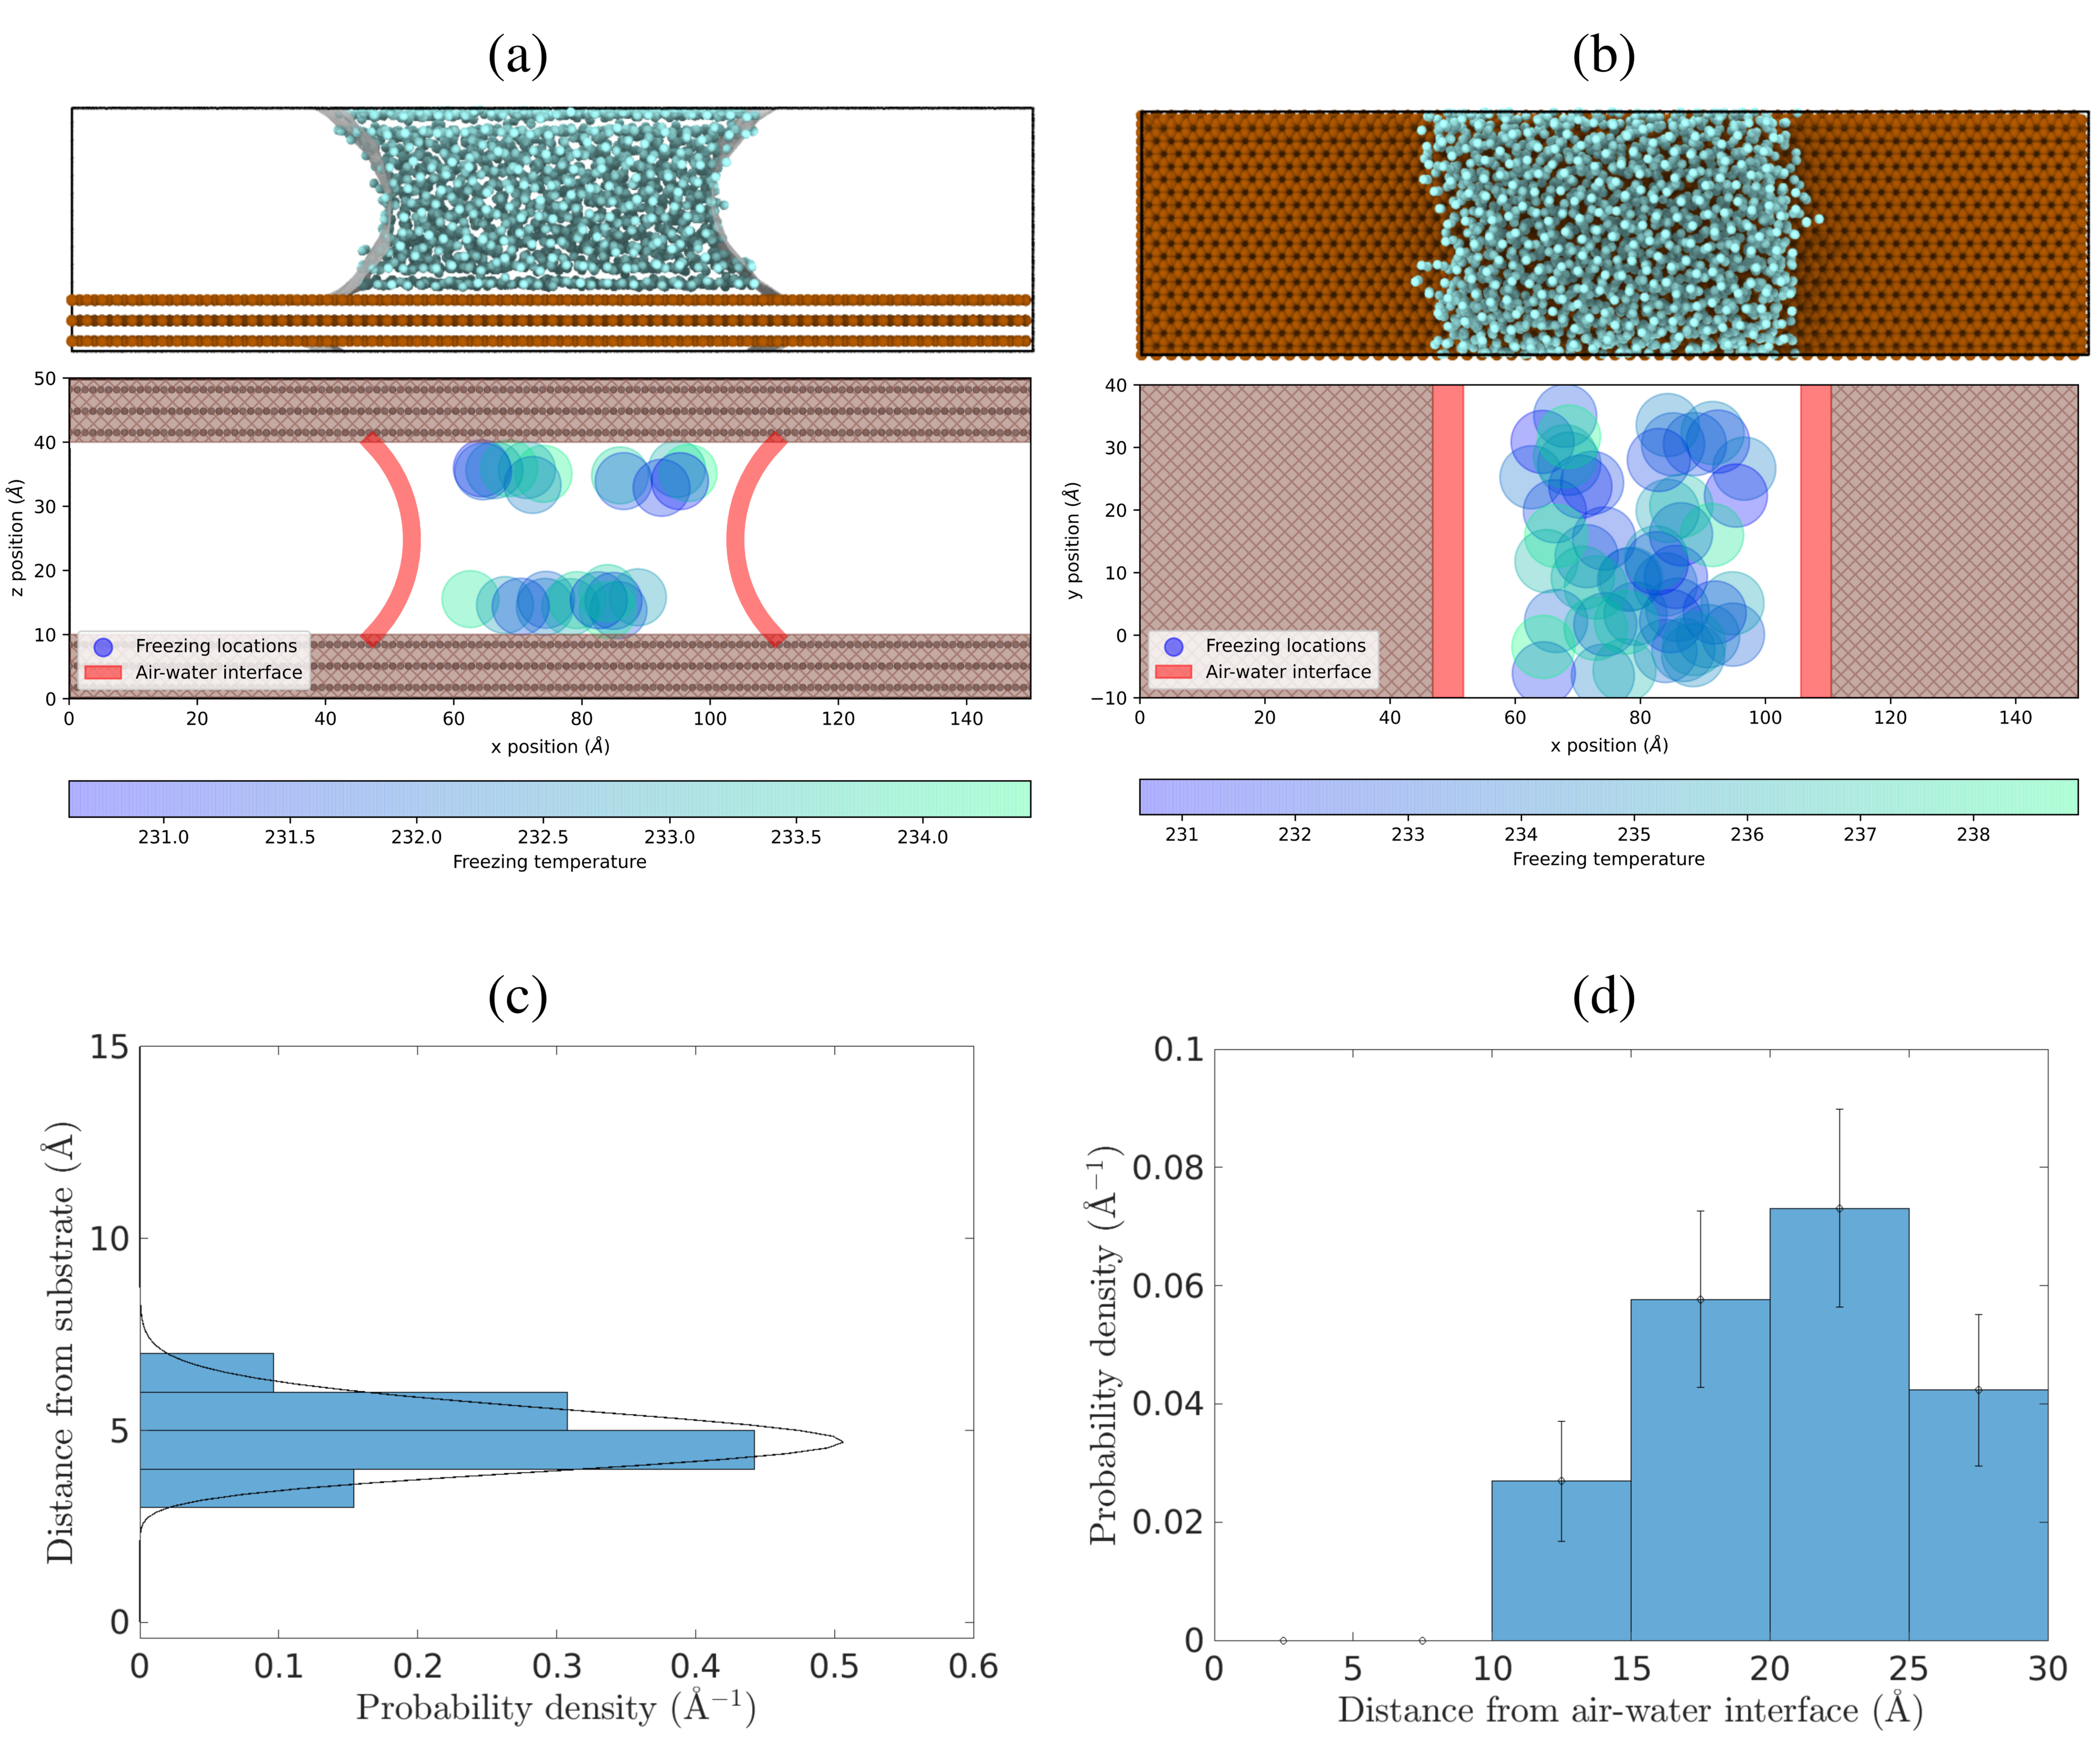
\includegraphics[width=12cm]{figures/freezing_locations_distributions.png}
%DIFDELCMD < %%%
\DIFdelendFL \DIFaddbeginFL \includegraphics[width=12cm]{figures/freezing_locations_distributions_revised.png}
\DIFaddendFL \caption{Spatial locations of ice nucleation within water capillary bridges. (a) Locations in a \DIFdelbeginFL \DIFdelFL{24 }\DIFdelendFL \DIFaddbeginFL \DIFaddFL{30 }\DIFaddendFL \AA{} tall capillary bridge, in the x-z plane. (b) Locations of freezing events in the x-y plane for both the 24 \AA{} and 30 \AA{} capillary bridges combined, viewed from above. (c) Probability density of ice nucleation initiating a distance away from the substrate, using \DIFdelbeginFL \DIFdelFL{data from }\DIFdelendFL \DIFaddbeginFL \DIFaddFL{freezing locations inside }\DIFaddendFL the 24 \AA{} and 30 \AA{} capillary bridges. The dashed line is a gamma distribution fit. (d) Probability density of ice nucleation initiating a distance away from the air-water interface (red shading in Fig. (a) and (b)) \DIFaddbeginFL \DIFaddFL{freezing locations inside the 24 \AA{} and 30 \AA{} capillary bridges}\DIFaddendFL .\label{fig:freezinglocations}}
\end{figure*}


\section{Discussion\DIFdelbegin \DIFdel{and Concluding Remarks}\DIFdelend }

From what we understand about ice nucleation, a supercooled water droplet in a cloud at a given temperature can be expected to freeze within a time frame dictated by the heterogeneous ice nucleation rate of the particle surfaces it may be in contact with. However, the factors that influence the heterogeneous nucleation rate are not all understood. Research on heterogeneous freezing in the atmosphere is performed on scales ranging from full clouds, using in-situ and remote sensing measurements to characterize aerosols and to identify the presence of ice in clouds; to the scale of single water droplets in laboratory studies and computer simulations to investigate the mechanisms that lead to freezing. Most measurements and computational results are interpreted in the context of classical nucleation theory, allowing the roles of temperature and time in the nucleation process to be understood \citep[e.g.,][]{niedermeier2011heterogeneous}. Most often, it is assumed that singular properties dominate over the stochastic time dependence, and it is therefore typical in cloud physics to characterize ice nucleating particles in terms of their freezing temperature \citep[e.g.,][]{hoose2012heterogeneous,frostenberg2022chance}. Knowledge of the freezing efficiency of ice nucleating particles is then used to understand the formation of ice in clouds \citep[e.g.,][]{yang2013minimalist,fu2017effect}. Their representation in coarse-resolution models even has implications for prediction of Arctic amplification in the climate problem \citep{tan2022potential}. 

This study has focused on how, for a fixed nucleation rate, the heterogeneous freezing temperature increases with decreasing pressure. Our key result is that the temperature corresponding to a certain ice nucleation rate increases linearly with the magnitude of negative pressure. Specifically, regardless of how negative pressure is created in the system, e.g. barostat or Laplace pressure, the change is described by the approximation $\Delta T/\Delta P = T_m \Delta v_{ls} / l_f$ (see Eq. (\ref{eq:dTdP})). This is certainly not true across a broad range of pressures \citep[e.g.,][]{bianco2021, espinosa2016}; however, for atmospheric processes it is likely that only the negative pressure range of 1 atm to $-1000$ atm, which was investigated here, is relevant. Therefore, the linear approximation can serve as the basis for a straightforward parameterization of the pressure effect. Essentially, the temperature increase for heterogeneous freezing is determined in large part by the volume difference between liquid and ice. For real water using the values listed in Table \ref{tab:slopes} we can estimate that the slope $(\Delta T/\Delta P)$ is $7.3 \times 10^{-8}$ K Pa$^{-1}$ $= 7.3 \times 10^{-3}$ K atm$^{-1}$. 
\DIFdelbegin \DIFdel{Consider, for example, a }\DIFdelend \DIFaddbegin 

\DIFadd{To understand the implications this pressure effect could have in atmospheric ice nucleation, consider a hypothetical }\DIFaddend case where atmospheric cloud droplets containing a certain type of \DIFdelbegin \DIFdel{ice nucleating particle }\DIFdelend \DIFaddbegin \DIFadd{ice-nucleating particle (IN) }\DIFaddend are likely to freeze within a second at $-20$ $^\circ$C\DIFdelbegin \DIFdel{, implying a corresponding }\DIFdelend \DIFaddbegin \DIFadd{. This would correspond to a }\DIFaddend nucleation rate of \DIFaddbegin \DIFadd{what we shall call }\DIFaddend $J_{atmospheric}$. The parameterization \DIFdelbegin \DIFdel{implied }\DIFdelend \DIFaddbegin \DIFadd{given }\DIFaddend by Eq. (\ref{eq:dTdP}) states that if the water in contact with the ice nucleating substrate is under a tension of $-500$ atm, then \DIFdelbegin \DIFdel{$\Delta T = 4$ }\DIFdelend \DIFaddbegin \DIFadd{$\Delta T_{het} \approx 3.7$ }\DIFaddend K. Thus, the same nucleation rate $J_{atmospheric}$ at which freezing occurs within a second, would instead be encountered at \DIFdelbegin \DIFdel{$-16$ }\DIFdelend \DIFaddbegin \DIFadd{$-16.3$ }\DIFaddend $^\circ$C. \DIFdelbegin \DIFdel{This negative pressure could be calculated according to the Laplace pressure, such that the environmental pressure can be 1 atm}\DIFdelend \DIFaddbegin \DIFadd{A common parameterization for the concentration of ice forming nuclei is $n_{IN} \propto \exp (\beta \delta T)$, where $\delta T = T_0 -T$ and $\beta \approx 0.6$ K$^{-1}$ \mbox{%DIFAUXCMD
\citep[Sec. 9.2]{pruppacher1997}}\hspace{0pt}%DIFAUXCMD
. It follows that the enhancement in the concentration of ice nucleating particles when pressure is reduced by $\Delta P$ is $n_{IN,\Delta P} / n_{IN} = \exp (\beta \Delta T)$, where $\Delta T$ is obtained from $\Delta P$ using Eq.~(\ref{eq:dTdP}). An order-of-magnitude increase in concentration results from $\Delta T = 3.8$ K, very close to the value suggested above for $-500$ atm. More recent measurements have led to refinements in parameterizations of $n_{IN}$}\DIFaddend , but the \DIFdelbegin \DIFdel{pressure within the water with a negative radius of curvature is negative}\DIFdelend \DIFaddbegin \DIFadd{general exponential trend with $\delta T$ still holds in many contexts \mbox{%DIFAUXCMD
\citep{demott2010predicting}}\hspace{0pt}%DIFAUXCMD
. Thus, these moderate differences in the temperature at which an IN is active are certainly worth attention in the context of mixed-phase clouds}\DIFaddend .

Natural examples abound with water under tension, having negative pressures in the range of 100s of atmospheres, within the range explored in this paper. For example, changes in pressure within mineral inclusions have been shown to lead to significant changes in the conditions for ice-water coexistence, and even to the superheating of ice \citep{roedder1967metastable}. Soils consist of a hierarchy of particle sizes that are bound through capillary tension, with similar pressure ranges being present \citep{seiphoori2020}. Negative pressures in trees, and even synthetic trees, reach negative pressures of 100s of atmospheres \citep{wheeler2008transpiration}. \DIFdelbegin \DIFdel{Our findings provide additional perspectives to those of \mbox{%DIFAUXCMD
\citet{lintunen2013anatomical}}\hspace{0pt}%DIFAUXCMD
, who showed a tendency for suppression of ice nucleation in the xylem of vascular plants. 
}%DIFDELCMD < 

%DIFDELCMD < %%%
\DIFdelend Negative pressures can also be generated through dynamic means. For example, droplets impacting solid or liquid surfaces can experience significant pressure perturbations \citep{cheng2022drop}. In fact, mechanical impact has been implemented as a method to initiate ice nucleation to avoid the persistence of supercooled liquid in phase-change thermal storage systems \citep{wang2022nucleation}. Conversely, imposing isochoric conditions has been shown to greatly increase the stability of supercooled water so that it can be used for cryopreservation \citep{powell2020isochoric}. One can speculate that there could be connections to contact nucleation or even formation of ice from collisions between supercooled droplets \citep{alkezweeny1969freezing} or breakup of supercooled raindrops that contain ice nucleating particles that otherwise would not be active, save for large, transient negative pressures \citep{james2021impact}. It has been observed repeatedly that ice generation in clouds is correlated with the presence of large drops \citep{rangno1991ice,lance2011cloud}, and it is worth noting that such drops are exactly what is needed to allow significant collisional growth or drop breakup. These will be exciting ideas to explore in future research.

Other perspectives on ice nucleation can also be related to the pressure and density-anomaly results presented here. \citet{baker2004new} argued that freezing in pure water occurs at the temperature at which its compressibility, with associated density fluctuations, reaches a maximum. The results were for atmospheric pressure, but the perspective that local densities of water and ice drive ice nucleation, rather than specific interfacial properties, is consistent. The effect of pressure on nucleation rate can be interpreted in terms of water activity; for example, \citep{knopf2013water} have shown via extensive laboratory experiments with a range of materials, that nucleation rates scale with water activity. This further extends the findings of \citet{koop2000water} that freezing and melting are related to pressure, following the water activity. The perspective of water activity dependence in aqueous solutions is most directly relevant to freezing temperature depression, but in general its dependence on pressure is consistent with our molecular dynamics results. Freezing temperature depression due to positive pressure in water was measured experimentally by \citet{kanno1975} and decrease in ice nucleation rate due to positive Laplace pressure in nano-scale water droplets was demonstrated by \citet{Li2013}, both leading to the intuitive notion that negative Laplace pressure will cause an increase in freezing temperature.

\DIFaddbegin \DIFadd{Creating Laplace pressures large enough in magnitude to enhance ice nucleation temperatures involves geometric configurations on nanometer spatial scales, which also may introduce confinement effects into the system. These considerations are important to understanding whether or not enhancement in ice nucleation can be expected. Experimental evidence in DSC experiments (Marcolli 2014) shows that no freezing enhancement was seen in confined pores, while \mbox{%DIFAUXCMD
\citet{lintunen2013anatomical} }\hspace{0pt}%DIFAUXCMD
show a tendency for ice nucleation to be suppressed in the xylem of vascular plants (which should be under significant negative pressure.) One important component in interpreting the discrepancy between these various findings is that experiments using cylindrical shaped pores are different from the confinement geometry found in slit pores. The key mechanism for rate enhancement in the slit pore configuration is the density oscillations induced by a flat interface (citation needed), which is destroyed by curved geometry.
}

\DIFadd{Even though the findings presented in this study describe the effect of negative pressure on heterogeneous ice nucleation rates, there are still open questions remaining that involve the thermodynamic properties of water at interfaces, under confinement, and across greater regions of waters phase diagram. Key questions of interest to refine and expand upon the results of this study include; (1) simulating different substrates to observe changes, if any, in the slope of heterogeneous nucleation rate coefficient lines, (2) exploring liquid water and ice properties near substrates to determine whether they alter the parameters in Eq.~\ref{eq:dTdP}, (3) assessing the level of surface freezing propensity present in the ML-mW water model and how this factors into the confinement effects seen in this study, and (4) investigating the interplay between cavitation and ice nucleation in this doubly metastable regime of water.
}


\DIFaddend % Concluding Remarks
\DIFaddbegin \section{\DIFadd{Concluding Remarks}}
\DIFaddend Using molecular dynamics simulations of heterogeneous ice nucleation on \DIFdelbegin \DIFdel{a hydrophilic }\DIFdelend \DIFaddbegin \DIFadd{an ice-nucleating }\DIFaddend substrate, we demonstrate that negative pressure within supercooled water allows for a given ice nucleation rate to occur at higher temperatures. The increase in \DIFaddbegin \DIFadd{heterogeneous }\DIFaddend freezing temperature with negative pressure \DIFdelbegin \DIFdel{is }\DIFdelend \DIFaddbegin \DIFadd{can be estimated as }\DIFaddend linear in nature, which lends support to the use of a linear approximation that depends on the latent heat release and \DIFdelbegin \DIFdel{water density anomaly }\DIFdelend \DIFaddbegin \DIFadd{the molar volume difference between liquid and ice }\DIFaddend to predict the slope. This approximation works particularly well for homogeneous nucleation rates; it is acceptable for heterogeneous nucleation, but \DIFdelbegin \DIFdel{the variables }\DIFdelend may need adjustment to provide better quantitative agreement.

To observe this pressure-dependent trend in heterogeneous nucleation rate, we first used a simulation setup with a substrate in contact with the volume of water. A barostat was applied to this system to probe pressures of 1 atm, $-500$ atm, and $-1000$ atm. Next, we created a configuration where negative pressure is introduced into the water without applying a barostat, but instead through negative Laplace pressure inside a water capillary bridge between \DIFdelbegin \DIFdel{two }\DIFdelend \DIFaddbegin \DIFadd{the }\DIFaddend surfaces of substrate. The pressure within the capillary \DIFaddbegin \DIFadd{bridge }\DIFaddend depends on the level of curvature, which is set by the contact angle and separation between substrate layers\DIFdelbegin \DIFdel{, and enhancement in }\DIFdelend \DIFaddbegin \DIFadd{. The observed enhancement in heterogeneous }\DIFaddend ice nucleation rate \DIFaddbegin \DIFadd{with increasing negative Laplace pressure is }\DIFaddend consistent with Eq. (\DIFdelbegin \DIFdel{\ref{eq:dTdP})was observed}\DIFdelend \DIFaddbegin \DIFadd{1)}\DIFaddend .

Finally, to see how confinement alone affects ice nucleation rate on the substrate, we decreased the \DIFaddbegin \DIFadd{substrate }\DIFaddend separation distance to 18, 24, and 30 \AA{}. We observed that 24 and 30-\AA{} separations showed identical ice nucleation rates as the larger volume system. The 18 \AA{} setup exhibited a large increase in ice nucleation rate as a result of the \DIFdelbegin \DIFdel{confined system}\DIFdelend \DIFaddbegin \DIFadd{confinement}\DIFaddend . Nucleation was also shown to avoid regions within approximately 10 \AA{} of an air-water interface\DIFdelbegin \DIFdel{, but may have a preference for that distance compared to the bulk}\DIFdelend . Thus, capillary bridges or other substrate-water geometries with layers less than 20 \AA{} thick will be strongly influenced by the proximity of the \DIFdelbegin \DIFdel{interface}\DIFdelend \DIFaddbegin \DIFadd{interfaces}\DIFaddend , and the simple parameterization of freezing temperature enhancement due to negative pressure cannot be directly applied.


\appendix
\section{Molecular Interaction Potential}\label{app: potential} 
%% Appendix A

Interactions between water molecules and other water molecules, as well as interactions between water molecules and substrate molecules are all described using versions of the Stillinger-Weber interaction potential \citep{stillinger1985computer}. When used for interactions involving water molecules, this potential is coarse-grained, meaning that the oxygen and hydrogen atoms are combined into one atom. The bonds between water molecules are then represented using a three-body potential, $\phi_{3}$, which is a function of the angle $\theta_{ijk}$ formed between every set of three water molecules ($i$,$j$, and $k$). This three-body potential creates a preference towards water \DIFdelbegin \DIFdel{molecuels adobpting }\DIFdelend \DIFaddbegin \DIFadd{molecules adopting }\DIFaddend a bond angle of approximately 105 degrees, set by the $\cos\theta_0$ parameter in Table \ref{Tab:potentials}. A two-body interaction term, $\phi_{2}$, applies forces that are dependent on the radial distance between two atoms $r_{ij}$.

\begin{align}\label{eq:sw-potential}
\phi_{2}(r_{ij}) &= A\epsilon\left[B(\frac{\sigma}{r_{ij}})^{p} - (\frac{\sigma}{r_{ij}})^{q}\right]\exp \left( \frac{\sigma}{r_{ij}-a\sigma}\right)\\
\phi_{3}(\theta_{ijk}, r_{ij}, r_{ik}) &= \lambda\epsilon[\cos\theta_{ijk} - \cos\theta_0]^2 \exp \left(\frac{\gamma\sigma}{r_{ij}-a\sigma}\right) \exp \left(\frac{\gamma\sigma}{r_{ik}-a\sigma}\right)
\end{align}

The parameters used for the interaction between water molecules and the substrate are summarized in Table \ref{Tab:potentials}. The cutoff distance where forces between molecules goes to zero is $a\sigma$. Note also that interactions between water molecules and substrate molecules do not have a three-body contribution, and are only influenced by the two-body potential term.

In creating a suitable interaction potential for an interaction between \DIFdelbegin \DIFdel{MLmW }\DIFdelend \DIFaddbegin \DIFadd{ML-mW }\DIFaddend water and the substrate, we start with the \DIFdelbegin \DIFdel{MLmW-MLmW }\DIFdelend \DIFaddbegin \DIFadd{ML-mW-ML-mW }\DIFaddend parameters and, as in the methods of \citet{fitzner2015facets}, only the $\epsilon$ and $\sigma$ values are adjusted to produce our \DIFdelbegin \DIFdel{MLmW-Substrate }\DIFdelend \DIFaddbegin \DIFadd{ML-mW--Substrate }\DIFaddend interaction. Given that the value of $\epsilon$ we have used is larger than that of the mW-Carbon interaction, the smaller contact angle that we see for \DIFdelbegin \DIFdel{MLmW-Substrate }\DIFdelend \DIFaddbegin \DIFadd{ML-mW--Substrate }\DIFaddend is consistent with \citet{Bi2016} and \citet{cox2015hydrophilicity}, where higher values of $\epsilon$ were used to increase hydrophilicity of the Carbon-mW interaction potential \cite{Bi2016}.

\appendixtables
\begin{table}
\DIFaddbeginFL \caption{\DIFaddFL{Parameters of the interaction potential between water and the substrate, and for water-water interactions, for the mW model and the ML-mW model. The Stillinger--Weber interaction potential is given by Eq. (\ref{eq:sw-potential}). }\label{Tab:potentials}}
\DIFaddendFL \begin{tabular}{ |p{1.95cm}||p{3.0cm}|p{3.0cm}|p{3.0cm}|p{3.0cm}|  }
 \hline
 & mW-Carbon  & \DIFdelbeginFL \DIFdelFL{MLmW-Substrate }\DIFdelendFL \DIFaddbeginFL \DIFaddFL{ML-mW--Substrate }\DIFaddendFL & mW-mW  &  \DIFdelbeginFL \DIFdelFL{MLmW-MLmW }\DIFdelendFL \DIFaddbeginFL \DIFaddFL{ML-mW-ML-mW }\DIFaddendFL \\
& \citep{lupi2014}  & & \citep{molinero2009} &  \citep{chan2019} \\
 \hline
 $\epsilon$ (Kcal/mole)    & 0.13          & 0.35      & 6.189         & 6.855473  \\
 $\sigma$ (\AA{})      & 3.2           & 2.2       & 2.3925        & 1.884015\\
 $a$                      & 1.80          & 2.124872  & 1.80          & 2.124872  \\
 $\lambda$                 & 0.0           & 0.0       & 23.15         & 24.673877 \\
 $\gamma$                  & 0.0           & 0.0       & 1.20          & 1.207943  \\
 $\cos\theta_0$              & 0.0           & 0.0       & $-0.33$         & $-0.279667$ \\
 $A$                      & 7.049556277   & 7.111598  & 7.049556277   & 7.111598  \\
 $B$                      & 0.6022245584  & 1.991526  & 0.6022245584  & 1.991526  \\
 $p$                      & 4.0           & 4.011214  & 4.0           & 4.011214  \\
 $q$                      & 0.0           & 0.0       & 0.0           & 0.0       \\
 $tol$                    & 0.0           & 0.0       & 0.0           & 0.0       \\
 \hline
\end{tabular}
\DIFdelbeginFL %DIFDELCMD < \caption{%
{%DIFAUXCMD
\DIFdelFL{Parameters of the interaction potential between water and the substrate, and for water-water interactions, for the mW model and the MLmW model. The Stillinger--Weber interaction potential is given by Eq. (\ref{eq:sw-potential}). }%DIFDELCMD < \label{Tab:potentials}%%%
}
%DIFAUXCMD
\DIFdelendFL \end{table}
\DIFaddbegin 

\section{\DIFadd{Freezing locations in an extra wide capillary}}\label{app: capillary} 
\DIFadd{Prompted by a reviewer comment, we constructed a 120 \AA{} wide capillary bridge to look at where in relation to the air-water interfaces ice nucleation events tend to occur. We see that they again avoid the immediate $\sim 10$ \AA{} vicinity of the air--water interface. However, the slight preference for freezing in the region just beyond 10 \AA{} from the air--water interface that was noticed in the 60 \AA{} wide capillary bridges is no longer pronounced in this 120 \AA{} wide capillary bridge. Oscillations in the density field may play a role here, making this an intriguing subject for further investigation.
}

\begin{figure*}[t]
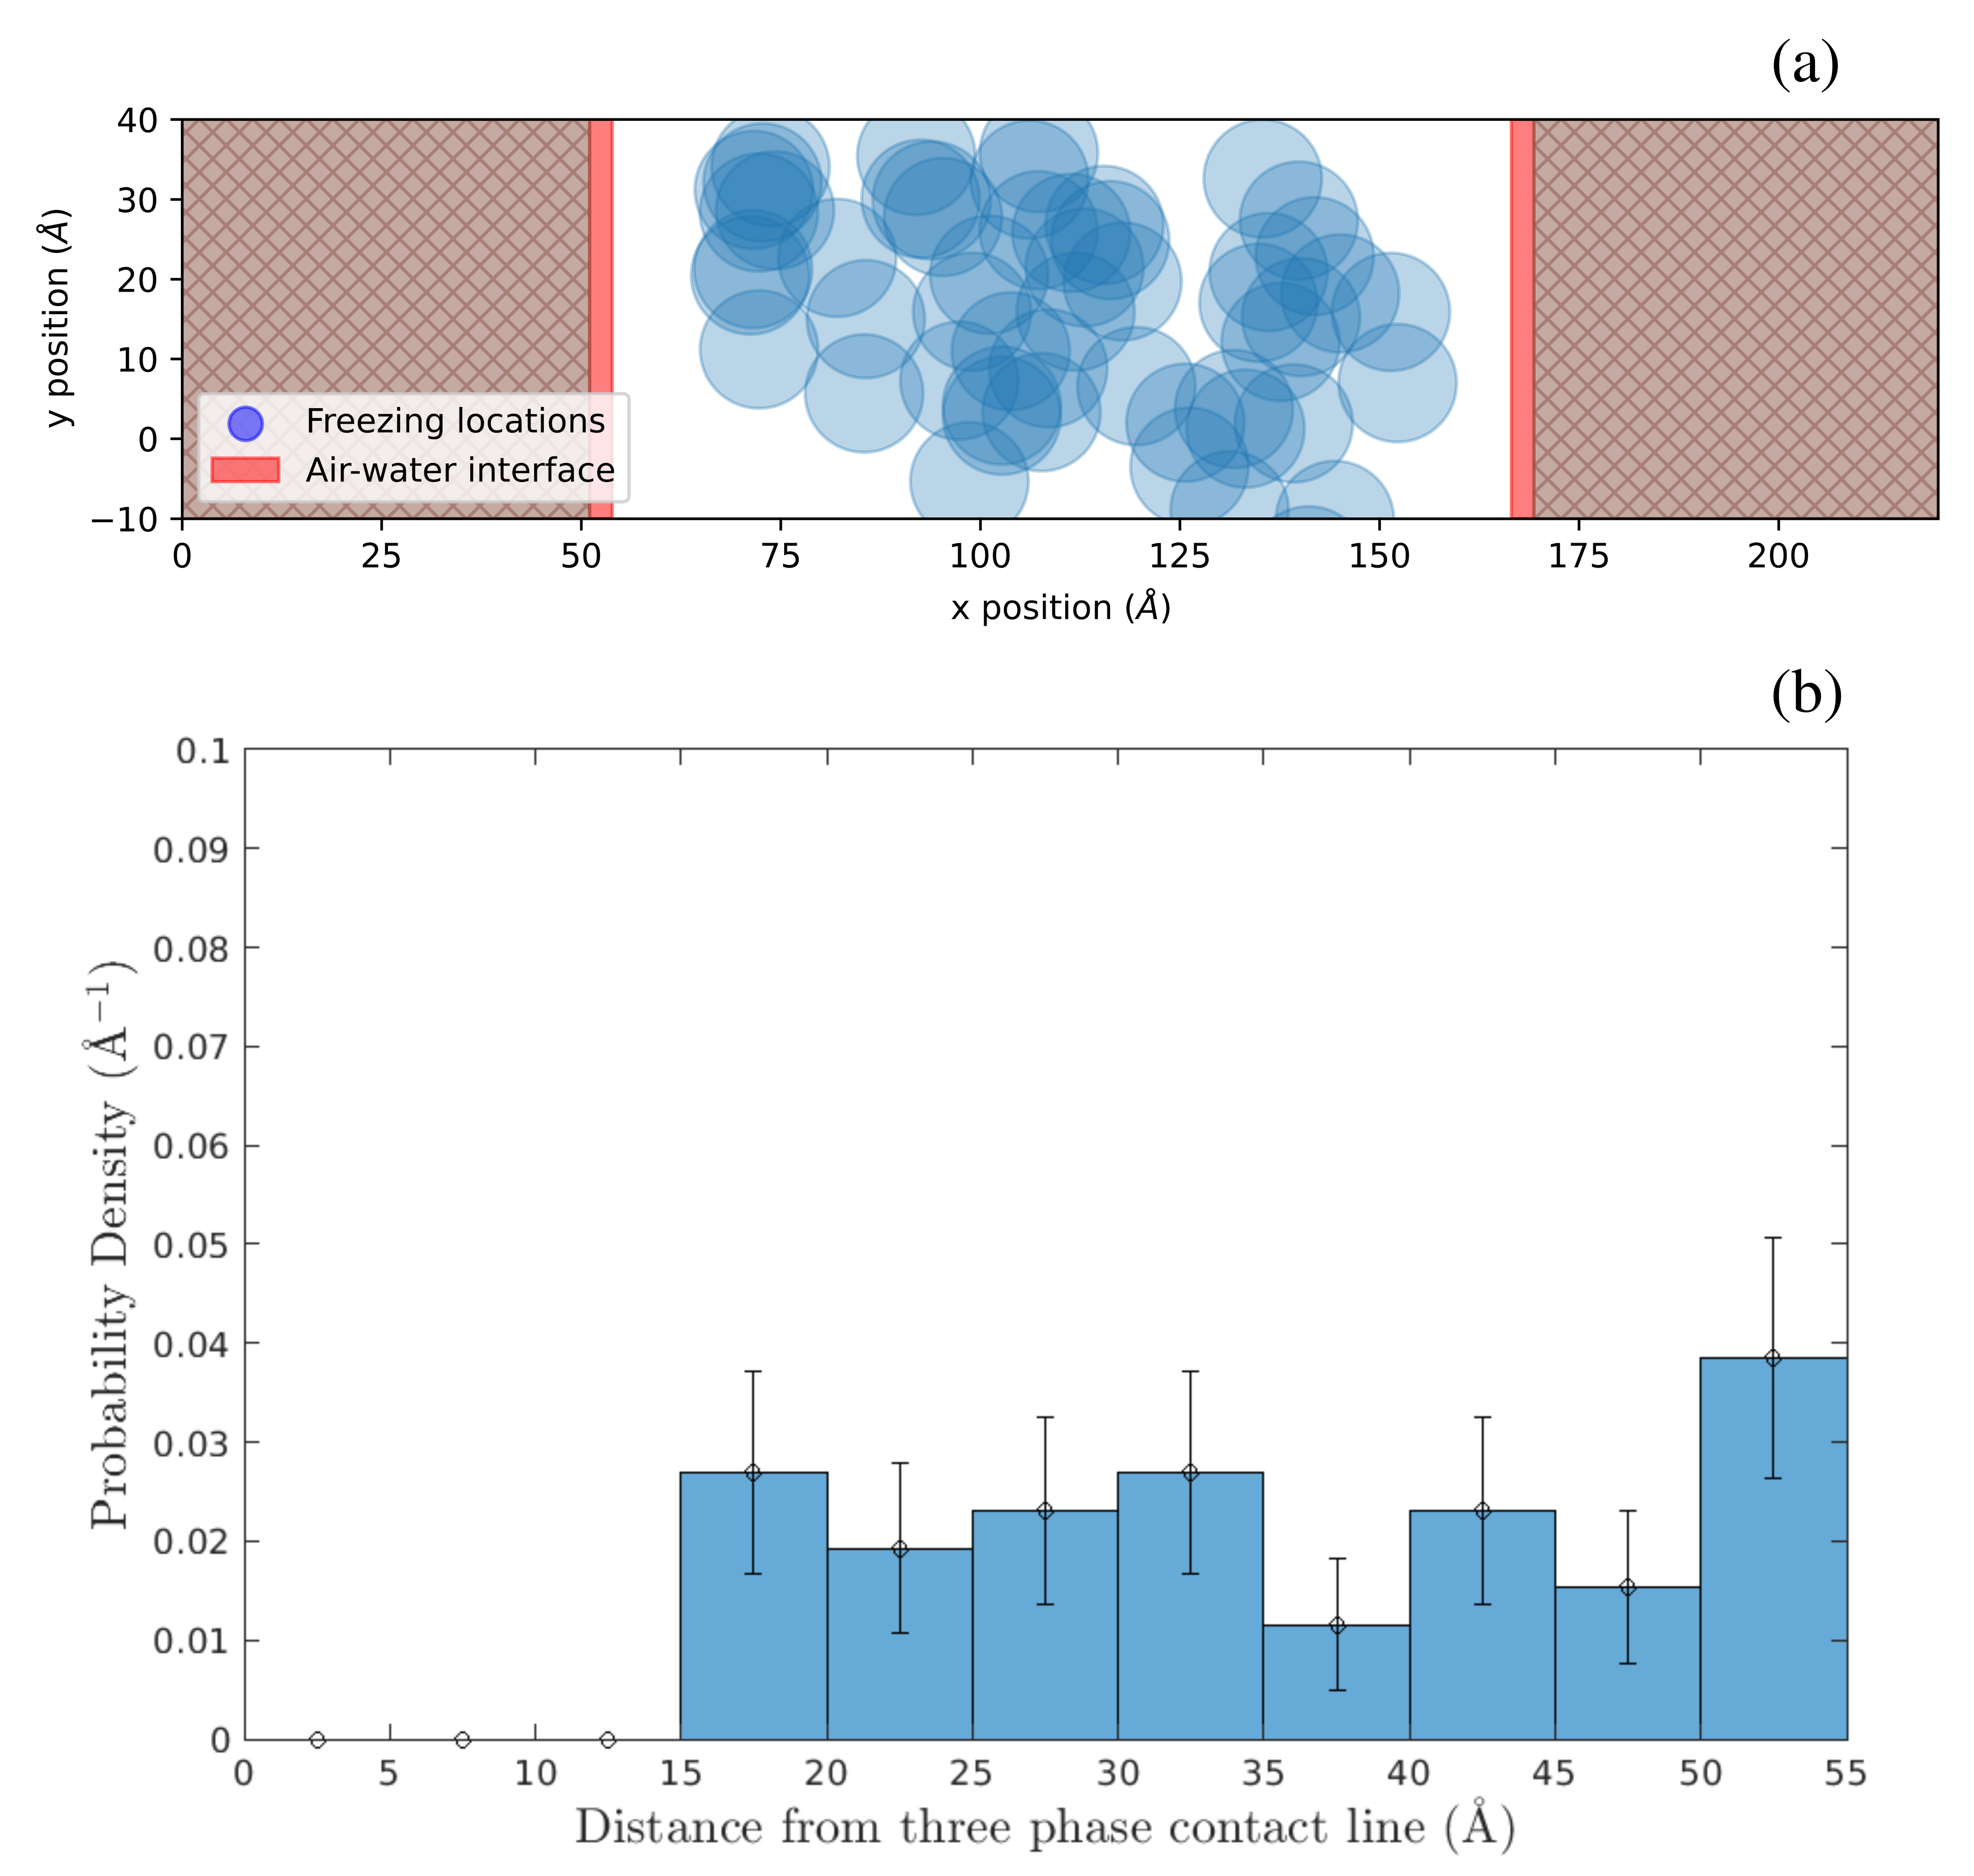
\includegraphics[width=12cm]{figures/appendix_freezing_distributions.png}
\caption{\DIFaddFL{(a) Ice nucleation locations in the x--y plane. (b) Probability distribution of freezing events as a function of distance from the nearest air-water interface in a 120 \AA{} wide capillary bridge.}}
\label{fig:appendix}
\end{figure*}
\DIFaddend 

%\subsection{}     %% Appendix A1, A2, etc.

\codedataavailability{
LAMMPS is free and open-source software developed by Sandia National Laboratory and a large user community. Scripts to reproduce simulations in LAMMPS and data going into Figures can be found at http://doi.org/10.37099/mtu.dc.all-datasets/41
} %% use this section when having data sets and software code available

\authorcontribution{ER, WC, and RAS designed the study; ER, TL, and IN set up the simulations; ER ran the simulations; All authors contributed to interpreting the results and writing the paper. 
} %% this section is mandatory

\competinginterests{No competing interests are present} %% this section is mandatory even if you declare that no competing interests are present

%\section{Acknowledgements}
\begin{acknowledgements}
Funding from NSF grant AGS-2019649 is gratefully acknowledged. TL acknowledges support from NSF through award CBET-2053330. IN acknowledges NSF (DMR-1944211). The High-Performance Computing Shared Facility (Portage) at Michigan Technological University was used in obtaining results presented in this publication. We acknowledge the LAMMPS community for helpful discussions and support.
\end{acknowledgements}

%\bibliography{references}
\bibliographystyle{copernicus}
\bibliography{references.bib}
\end{document}













